% Báo cáo phần việc TV2 - Bài tập lớn Tính toán tiến hoá
% Biên dịch: xelatex bao_cao_tv2.tex (chạy 2 lần để có mục lục, danh mục hình/bảng)
\documentclass[a4paper,fontsize=13pt,oneside,listof=totoc,bibliography=totoc,
               headings=normal,numbers=noenddot]{scrreprt}

% ----------------------------------------------------------------- thông tin sinh viên (điền)
\newcommand{\TenTruong}{TRƯỜNG CÔNG NGHỆ THÔNG TIN VÀ TRUYỀN THÔNG}
\newcommand{\HocPhan}{TÍNH TOÁN TIẾN HOÁ}
\newcommand{\TenSV}{[Họ và tên sinh viên]}
\newcommand{\MSSV}{[Mã số sinh viên]}
\newcommand{\Lop}{[Mã lớp học phần]}
\newcommand{\GVHD}{[Họ tên giảng viên]}
\newcommand{\Nhom}{[Tên nhóm]}

% ----------------------------------------------------------------- trang, font, ngôn ngữ
\usepackage[left=3cm,right=2cm,top=2.5cm,bottom=2.5cm]{geometry}
\usepackage{fontspec}
\setmainfont{Times New Roman}
\setmonofont[Scale=0.85]{Consolas}
\usepackage[vietnamese]{babel}
\usepackage{setspace}
\setstretch{1.3}
\usepackage{indentfirst}
\setlength{\parindent}{1cm}
\setlength{\parskip}{4pt}

% ----------------------------------------------------------------- tiêu đề chương, mục
\RedeclareSectionCommand[beforeskip=0pt,afterskip=1.2\baselineskip]{chapter}
\renewcommand*{\raggedchapter}{\centering}
\renewcommand*{\chapterformat}{\MakeUppercase{\chaptername}~\thechapter.\enskip}
\renewcommand*{\chapterlinesformat}[3]{#2#3}
\setkomafont{disposition}{\rmfamily\bfseries}
\setkomafont{chapter}{\rmfamily\bfseries\fontsize{15}{19}\selectfont}
\setkomafont{section}{\rmfamily\bfseries\fontsize{14}{17}\selectfont}
\setkomafont{subsection}{\rmfamily\bfseries\itshape\fontsize{13}{16}\selectfont}
\setcounter{secnumdepth}{3}
\setcounter{tocdepth}{2}

% ----------------------------------------------------------------- toán, bảng, hình
\usepackage{amsmath,mathtools}
\usepackage{unicode-math}
\setmathfont{TeX Gyre Termes Math}
\usepackage{graphicx}
\graphicspath{{hinh/}}
\usepackage{booktabs,multirow,array,tabularx,longtable}
\usepackage{xcolor}
\definecolor{hustred}{HTML}{C8102E}
\definecolor{blue1}{HTML}{2a78d6}
\definecolor{orange1}{HTML}{eb6834}
\definecolor{aqua1}{HTML}{1baf7a}
\definecolor{yellow1}{HTML}{eda100}
\definecolor{grayline}{HTML}{8a8a85}
\usepackage[font=small,labelfont=bf,labelsep=period,justification=centering]{caption}
\usepackage{subcaption}
\usepackage{float}
\usepackage{tikz}
\usetikzlibrary{arrows.meta,positioning,shapes.geometric,calc,fit,backgrounds}
\usepackage{pgfplots}
\pgfplotsset{compat=1.18}
\usepgfplotslibrary{groupplots}
\usepackage[linesnumbered,ruled,vlined]{algorithm2e}
\SetAlgorithmName{Thuật toán}{thuật toán}{Danh mục thuật toán}
\SetKwInput{KwIn}{Đầu vào}
\SetKwInput{KwOut}{Đầu ra}
\SetAlFnt{\small}
\usepackage{fancyvrb}
\fvset{frame=single,framesep=5pt,fontsize=\small,rulecolor=\color{grayline}}
\usepackage{listings}
\lstset{basicstyle=\ttfamily\small,breaklines=true,frame=single,framerule=0.4pt,
        rulecolor=\color{grayline},columns=fullflexible,keepspaces=true,extendedchars=true}
\usepackage{enumitem}
\setlist{itemsep=2pt,topsep=4pt}
\usepackage{siunitx}
\sisetup{output-decimal-marker={,},group-separator={.},group-minimum-digits=4}
\usepackage[hidelinks]{hyperref}

% ----------------------------------------------------------------- đầu trang, chân trang
\usepackage[headsepline=0.4pt]{scrlayer-scrpage}
\clearpairofpagestyles
\ihead{\small\itshape Báo cáo phần việc TV2: khởi tạo thông minh và tìm kiếm cục bộ}
\cfoot*{\pagemark}
\renewcommand*{\chapterpagestyle}{plain.scrheadings}

\newcommand{\code}[1]{\texttt{#1}}

\begin{document}
\begin{titlepage}
\newgeometry{left=2.5cm,right=2.5cm,top=2cm,bottom=2cm}
\begin{tikzpicture}[remember picture,overlay]
  \draw[line width=2.5pt,color=hustred]
    ($(current page.north west)+(1.5cm,-1.5cm)$) rectangle ($(current page.south east)+(-1.5cm,1.5cm)$);
  \draw[line width=0.6pt,color=hustred]
    ($(current page.north west)+(1.7cm,-1.7cm)$) rectangle ($(current page.south east)+(-1.7cm,1.7cm)$);
\end{tikzpicture}
\centering
\setstretch{1.2}
{\fontsize{15}{18}\selectfont\bfseries ĐẠI HỌC BÁCH KHOA HÀ NỘI\par}
{\fontsize{13}{16}\selectfont\bfseries \TenTruong\par}
\vspace{0.3cm}
\rule{0.4\textwidth}{0.6pt}\par
\vspace{0.9cm}

\includegraphics[height=4.2cm]{logo_hust.png}\par
\vspace{1.1cm}
{\fontsize{20}{24}\selectfont\bfseries BÁO CÁO BÀI TẬP LỚN\par}
\vspace{0.3cm}
{\fontsize{14}{17}\selectfont\bfseries HỌC PHẦN: \HocPhan\par}
\vspace{1cm}
{\fontsize{16}{21}\selectfont\bfseries\color{hustred}
 THUẬT TOÁN NSGA-II CHO BÀI TOÁN\\ ĐỊNH TUYẾN XE XANH ĐA MỤC TIÊU\\ CÓ KHUNG THỜI GIAN (MOGVRPTW)\par}
\vspace{0.6cm}
{\fontsize{14}{18}\selectfont\bfseries Phần việc TV2: Khởi tạo quần thể thông minh\\
 và tìm kiếm cục bộ trong tuyến\par}
\vfill
\begin{tabular}{@{}l@{\hspace{0.6cm}}l@{}}
  \textbf{Sinh viên thực hiện:} & \TenSV \\
  \textbf{Mã số sinh viên:}     & \MSSV \\
  \textbf{Lớp:}                 & \Lop \\
  \textbf{Nhóm:}                & \Nhom \\
  \textbf{Giảng viên hướng dẫn:} & \GVHD \\
\end{tabular}
\vfill
{\fontsize{13}{16}\selectfont\bfseries HÀ NỘI, THÁNG 11/2026\par}
\restoregeometry
\end{titlepage}


\pagenumbering{roman}
\chapter*{LỜI MỞ ĐẦU}
\addcontentsline{toc}{chapter}{Lời mở đầu}

Bài tập lớn của nhóm cài đặt thuật toán NSGA-II cho bài toán định tuyến xe xanh đa mục tiêu có khung
thời gian (MOGVRPTW), dựa trên mô hình của bài báo Li và cộng sự năm 2025~\cite{li2025}. Bài toán có ba mục tiêu xung
đột nhau: chi phí giao hàng, lượng khí thải CO\textsubscript{2} và mức hài lòng của khách hàng. Sau khi
có thuật toán gốc, nhóm bổ sung bốn cải tiến. Mỗi cải tiến do một thành viên phụ trách, có cờ bật tắt
riêng trong tệp cấu hình và mặc định ở trạng thái tắt, để có thể đo đóng góp của từng cải tiến.

Báo cáo này trình bày phần việc của thành viên thứ hai (TV2) gồm hai cải tiến: khởi tạo quần thể thông
minh (\code{init\_smart}) và tìm kiếm cục bộ trong từng tuyến (\code{local\_search}). Ngoài hai mô-đun
thuật toán, phần việc còn gồm bộ kiểm thử, gắn cải tiến vào vòng lặp NSGA-II của nhóm, kiểm tra hồi
quy để bảo đảm khi tắt cờ thì kết quả trùng khớp với thuật toán gốc, chạy thực nghiệm so sánh trên
nhiều bộ dữ liệu và vẽ các biểu đồ kết quả.

Nội dung được trình bày theo thứ tự: bài toán và nhiệm vụ của TV2 (Chương~1), cơ sở lý thuyết
(Chương~2), thiết kế và cài đặt khởi tạo thông minh (Chương~3), thiết kế và cài đặt tìm kiếm cục bộ
(Chương~4), tích hợp vào NSGA-II và kiểm thử (Chương~5), thực nghiệm (Chương~6), tiến độ cùng những
việc còn cần hoàn thiện (Chương~7). Mọi số liệu trong báo cáo được lấy từ các lần chạy thật trên mã
nguồn của nhóm; cách tái lập từng bảng và từng hình được ghi ở phần phụ lục.

\tableofcontents
\listoffigures
\listoftables
\chapter*{DANH MỤC TỪ VIẾT TẮT VÀ KÝ HIỆU}
\addcontentsline{toc}{chapter}{Danh mục từ viết tắt và ký hiệu}

\begin{longtable}{@{}p{3.2cm}p{11.3cm}@{}}
\toprule
\textbf{Viết tắt} & \textbf{Ý nghĩa} \\
\midrule
\endhead
MOGVRPTW & Multi-Objective Green Vehicle Routing Problem with Time Windows: bài toán định tuyến xe xanh
           đa mục tiêu có khung thời gian \\
NSGA-II  & Non-dominated Sorting Genetic Algorithm II: giải thuật di truyền sắp xếp không trội, phiên bản 2 \\
NN       & Nearest Neighbor: láng giềng gần nhất \\
TW       & Time Window: khung thời gian; trong báo cáo dùng để chỉ cách khởi tạo theo thứ tự khung giờ \\
LS       & Local Search: tìm kiếm cục bộ \\
OX       & Order Crossover: lai ghép thứ tự \\
DP       & Dynamic Programming: quy hoạch động (cách cắt tuyến tối ưu của TV4) \\
HV       & Hypervolume: thể tích vùng bị trội \\
IGD      & Inverted Generational Distance: khoảng cách thế hệ đảo \\
SP       & Spacing: độ đều của tập nghiệm \\
SC       & Set Coverage: độ phủ tập \\
RNG      & Random Number Generator: bộ sinh số ngẫu nhiên \\
TV1--TV4 & Thành viên 1 đến thành viên 4 của nhóm \\
\midrule
\textbf{Ký hiệu} & \textbf{Ý nghĩa} \\
\midrule
$n$                     & số khách hàng (không tính kho, kho có chỉ số 0) \\
$\pi$                   & hoán vị khách hàng, là nhiễm sắc thể của một cá thể \\
$Q$                     & tải trọng tối đa của một xe (kg) \\
$K$                     & số xe tối đa của đội xe (\code{fleet\_size}) \\
$d_{ij}$                & khoảng cách Euclid giữa điểm $i$ và $j$ (km) \\
$[ET_i, LT_i]$          & khung thời gian chấp nhận được của khách $i$ \\
$[ETa_i, LTb_i]$        & khung thời gian kỳ vọng của khách $i$, nằm bên trong $[ET_i, LT_i]$ \\
$f_1, f_2, f_3$         & chi phí (CNY), khí thải CO\textsubscript{2} (kg), mức hài lòng trung bình (0--1) \\
$\mathbf{g}$            & vectơ mục tiêu cực tiểu hoá $(f_1, f_2, 1-f_3)$ \\
$N_{pop}$, $G$          & kích thước quần thể, số thế hệ \\
$p_c$, $p_m$, $p_{ls}$  & xác suất lai ghép, đột biến, chạy tìm kiếm cục bộ \\
$\mathbf{w}$, $\mathbf{s}$ & vectơ trọng số và vectơ hệ số chuẩn hoá trong tiêu chí tổng có trọng số \\
\bottomrule
\end{longtable}


\cleardoublepage
\pagenumbering{arabic}
\chapter{TỔNG QUAN BÀI TOÁN VÀ NHIỆM VỤ CỦA TV2}
\label{chap:tongquan}

\section{Bài toán định tuyến xe xanh đa mục tiêu có khung thời gian}

Một công ty có một kho hàng và một đội xe tải giống nhau, cần giao hàng cho $n$ khách. Mỗi khách $i$
có toạ độ, lượng hàng cần nhận $q_i$, thời gian dỡ hàng $s_i$ và hai khung thời gian lồng nhau: khung kỳ
vọng $[ETa_i, LTb_i]$ là khoảng khách muốn nhận hàng nhất, khung chấp nhận được $[ET_i, LT_i]$ rộng hơn,
ngoài khung này khách không hài lòng chút nào. Mỗi xe xuất phát từ kho, đi qua một số khách theo một thứ
tự rồi quay về kho. Tổng lượng hàng trên một xe không vượt quá tải trọng $Q$, và số xe dùng không vượt
quá $K$. Lời giải là cách chia khách cho các xe và thứ tự ghé thăm trên từng xe.

Bài toán có ba mục tiêu cùng lúc:
\begin{itemize}
  \item $f_1$: tổng chi phí giao hàng (CNY), cần cực tiểu;
  \item $f_2$: tổng lượng khí thải CO\textsubscript{2} (kg), cần cực tiểu;
  \item $f_3$: mức hài lòng trung bình của khách, trong đoạn $[0,1]$, cần cực đại.
\end{itemize}
Ba mục tiêu này xung đột nhau. Dùng thêm xe giúp đến đúng giờ hơn (tăng $f_3$, giảm phạt trễ trong $f_1$)
nhưng làm tăng chi phí cố định và quãng đường (tăng $f_2$). Vì vậy kết quả không phải một lời giải duy
nhất mà là một tập lời giải không trội nhau, gọi là tập Pareto.

\subsection{Ba hàm mục tiêu}

Các tham số được lấy theo bảng 2 của bài báo gốc và ghi trong \code{config.yaml}.

\paragraph{Chi phí $f_1$.} Gồm bốn thành phần:
\begin{equation}
  f_1 = F_1 + F_2 + F_3 + F_4 .
\end{equation}
$F_1 = \sigma_1 \cdot \text{Fuel}$ là tiền nhiên liệu, với $\sigma_1 = 10$ CNY/lít. Suất tiêu thụ trên
một chặng phụ thuộc tải hiện có trên xe trước khi giao cho khách tiếp theo:
\begin{equation}
  \rho(L) = \rho_0 + \frac{\rho^* - \rho_0}{Q}\, L ,
  \qquad \rho_0 = 0{,}122 \text{ L/km},\; \rho^* = 0{,}388 \text{ L/km},
\end{equation}
nên lượng nhiên liệu của chặng dài $d$ là $d\cdot\rho(L)$. $F_2 = \sigma_2 m$ là chi phí cố định cho
$m$ xe được dùng ($\sigma_2 = 100$ CNY/xe). $F_3 = \sigma_3 \sum d$ là chi phí theo quãng đường
($\sigma_3 = 2$ CNY/km). $F_4$ là tiền phạt lệch khung kỳ vọng:
\begin{equation}
  F_4 = \frac{\alpha \sum_i \max(ETa_i - t_i, 0) + \beta \sum_i \max(t_i - LTb_i, 0)}{60},
\end{equation}
với $t_i$ là giờ xe đến khách $i$ tính bằng phút, $\alpha = 20$ CNY/giờ cho đến sớm, $\beta = 60$
CNY/giờ cho đến muộn. Phép chia cho 60 đổi số phút sang giờ.

\paragraph{Khí thải $f_2$.} Theo mô hình MEET, với vận tốc không đổi $v = 40$ km/h:
\begin{equation}
  f_2 = \frac{\varphi(v)\,\psi(v)}{1000} \sum d, \qquad
  \varphi(v) = c_0 + c_1 v^3 + \frac{c_2}{v}, \qquad
  \psi(v) = d_0 + d_1 v + d_2 v^2 + \frac{d_3}{v}.
\end{equation}
Bài báo in số hạng $d_2 v^3$ khiến $\psi$ âm ở $v = 40$; nhóm sửa thành $d_2 v^2$, khi đó mỗi km thải
khoảng $679{,}44$ g CO\textsubscript{2}. Hệ quả quan trọng là $f_2$ tỉ lệ thuận với tổng quãng đường,
nên $f_2$ và thành phần $F_3$ của $f_1$ biến thiên cùng chiều.

\paragraph{Mức hài lòng $f_3$.} Mỗi khách có hàm hài lòng hình thang $W_i(t)$, thang 0--100:
\begin{equation}
  W_i(t) =
  \begin{cases}
    0 & t < ET_i \text{ hoặc } t > LT_i,\\[2pt]
    100\,\dfrac{t - ET_i}{ETa_i - ET_i} & ET_i \le t < ETa_i,\\[6pt]
    100 & ETa_i \le t \le LTb_i,\\[2pt]
    100\,\dfrac{LT_i - t}{LT_i - LTb_i} & LTb_i < t \le LT_i,
  \end{cases}
  \qquad
  f_3 = \frac{1}{n}\sum_{i=1}^{n} \frac{W_i(t_i)}{100}.
\end{equation}
Nhóm tính $W$ tại giờ xe đến (\code{satisfaction\_time: arrival}). Xe đến sớm thì chờ tới $ETa_i$ rồi
mới dỡ hàng.

\subsection{Dữ liệu}

Nhóm dùng bộ Solomon~\cite{solomon1987} (bản 100 khách, lấy $n$ khách đầu cho các cỡ 25 và 50), tải trọng $Q = 400$ kg,
đội xe tối đa $K = 25$, khung chấp nhận được là khung gốc nới thêm 30 phút mỗi đầu. Ngoài ra có bộ dữ
liệu thực tế 29 khách (\code{case29}) từ bảng 8 của bài báo, tải trọng 4000 kg, chưa giới hạn số xe.
Phần việc của TV2 thực nghiệm trên bốn instance đại diện: C102-25 (khách phân cụm, khung hẹp), R201-50
(phân bố ngẫu nhiên, khung rộng), RC201-100 (hỗn hợp, cỡ lớn) và case29-29 (dữ liệu thực tế).

\section{Mã hoá lời giải và bộ giải mã}
\label{sec:decoder}

Một cá thể là một hoán vị $\pi$ của các khách $1,\dots,n$, không chứa kho. Bộ giải mã (\code{decoder.py})
cắt hoán vị thành các tuyến theo đúng thứ tự trong hoán vị. Nhóm dùng quy tắc cắt
\code{capacity\_time}: đi dọc hoán vị, mở tuyến mới khi khách tiếp theo làm xe vượt tải, hoặc khi xe sẽ
đến khách tiếp theo sau $LT$ mà đội xe vẫn còn xe trống. Sau khi cắt, bộ giải mã đi dọc từng tuyến, tính
giờ đến, tải, quãng đường rồi ra $(f_1, f_2, f_3)$ cùng các thông tin phụ như danh sách tuyến, số xe và
cờ \code{fleet\_ok} cho biết số xe có vượt $K$ hay không.

Cách mã hoá này luôn cho lời giải hợp lệ về tải, nhưng có một hệ quả mà phần tìm kiếm cục bộ phải xử lý:
chỗ cắt tuyến phụ thuộc vào toàn bộ thứ tự trong hoán vị. Đổi thứ tự khách bên trong một tuyến có thể
làm chỗ cắt dịch đi, tức bộ giải mã tạo ra một bộ tuyến khác (mục~\ref{sec:drift}).

\section{Thuật toán NSGA-II của nhóm}

TV1 cài đặt NSGA-II gốc trong \code{src/nsga2.py}. Quần thể có $N_{pop} = 80$ cá thể, chạy $G = 200$
thế hệ. Mỗi thế hệ: chọn cha mẹ bằng giải đấu nhị phân theo hạng và khoảng cách đông đúc, lai ghép thứ
tự (OX) với xác suất $p_c = 0{,}7$, đột biến đảo đoạn hoặc hoán đổi hai vị trí với xác suất
$p_m = 0{,}1$ (Solomon) hoặc $0{,}2$ (case29), đánh giá con, gộp cha mẹ với con rồi chọn lọc môi trường
theo front và khoảng cách đông đúc, có loại các hoán vị trùng nhau. Ràng buộc số xe được xử lý bằng trội
có ràng buộc: lời giải vượt ít xe hơn luôn thắng. Toàn bộ thuật toán dùng một bộ sinh số ngẫu nhiên
\code{np.random.default\_rng(seed)} duy nhất, nên cùng seed luôn cho cùng kết quả.

\section{Bốn cải tiến và nhiệm vụ của TV2}

\begin{table}[H]
\centering
\caption{Bốn cải tiến của nhóm và người phụ trách}
\label{tab:caitien}
\begin{tabularx}{\textwidth}{@{}lXl@{}}
\toprule
\textbf{Cải tiến} & \textbf{Ý tưởng} & \textbf{Người làm} \\
\midrule
\code{init\_smart}   & khởi tạo quần thể bằng láng giềng gần nhất, sắp theo khung giờ và ngẫu nhiên & TV2 \\
\code{local\_search} & 2-opt và Or-opt trên từng tuyến sau đột biến & TV2 \\
\code{diversity}     & SDE hoặc mật độ kNN thay khoảng cách đông đúc, thêm kho lưu trữ ngoài & TV3 \\
\code{dp\_split}, \code{adaptive\_rates} & cắt tuyến tối ưu bằng quy hoạch động; $p_c$, $p_m$ thích nghi & TV4 \\
\bottomrule
\end{tabularx}
\end{table}

Theo phân công trong README của nhóm, TV2 phải làm các việc sau.
\begin{enumerate}
  \item \textbf{Giai đoạn 2 (12/11--18/11).} Cài đặt \code{init\_smart} và \code{local\_search}, mỗi cải
        tiến một tệp trong \code{src/improvements/}, bật tắt bằng một cờ trong \code{config.yaml}, mặc định
        tắt. Viết test riêng. Chứng minh khi tắt cờ thì ra đúng kết quả của thuật toán gốc với cùng seed.
        Chạy 10 seed trên ít nhất 3 instance và so HV với thuật toán gốc.
  \item \textbf{Giai đoạn 3 (19/11--25/11).} Hỗ trợ ghép các nhánh, chuẩn bị mốc hồi quy: tắt hết cờ phải
        ra đúng từng con số như thuật toán gốc.
  \item \textbf{Giai đoạn 4 (26/11--02/12).} Vẽ biểu đồ: front Pareto ba chiều, đường hội tụ HV, biểu đồ
        hộp HV và IGD qua 10 seed.
\end{enumerate}

Ngoài ra có bốn quy tắc chung bắt buộc cho mọi cải tiến: (i) cờ tắt thì code cải tiến không được gọi
bộ sinh số ngẫu nhiên lần nào, (ii) chỉ dùng bộ sinh do \code{nsga2.run} truyền vào, (iii) mọi tham số
đặt trong \code{config.yaml} dưới mục \code{improvements}, (iv) mọi lần đánh giá thêm phải được cộng vào
số lần đánh giá \code{n\_evals}, để so sánh giữa các cấu hình được công bằng.

Riêng với tìm kiếm cục bộ, README nêu sẵn một điểm phải cẩn thận: sau khi cải thiện một tuyến rồi nối
các tuyến lại thành hoán vị, bộ giải mã cắt lại có thể ra bộ tuyến khác, khiến phần cải thiện bị mất
hoặc bị tính sai. Chương~\ref{chap:ls} trình bày cách xử lý điểm này.

\chapter{CƠ SỞ LÝ THUYẾT}
\label{chap:coso}

\section{Tối ưu đa mục tiêu và quan hệ trội Pareto}

Để so sánh lời giải theo cùng một chiều, nhóm đưa ba mục tiêu về dạng cùng cực tiểu hoá:
\begin{equation}
  \mathbf{g}(\pi) = \big(g_1, g_2, g_3\big) = \big(f_1(\pi),\; f_2(\pi),\; 1 - f_3(\pi)\big).
\end{equation}
Lời giải $a$ \emph{trội} lời giải $b$, ký hiệu $a \prec b$, khi $a$ không tệ hơn $b$ ở mọi mục tiêu và
tốt hơn hẳn ở ít nhất một mục tiêu:
\begin{equation}
  a \prec b \iff \forall k:\ g_k(a) \le g_k(b) \;\;\text{và}\;\; \exists j:\ g_j(a) < g_j(b).
\end{equation}
Tập các lời giải không bị lời giải nào trội gọi là tập Pareto; ảnh của nó trong không gian mục tiêu
gọi là mặt Pareto (front). Mục đích của thuật toán là tìm một tập xấp xỉ mặt Pareto vừa gần mặt thật,
vừa trải đều.

Trong phần tìm kiếm cục bộ, phép so sánh dùng thêm một sai số $\varepsilon \ge 0$ để tránh chấp nhận
các thay đổi chỉ do sai số làm tròn số thực:
\begin{equation}
  a \prec_\varepsilon b \iff \forall k:\ g_k(a) \le g_k(b) + \varepsilon \;\;\text{và}\;\;
  \exists j:\ g_j(a) < g_j(b) - \varepsilon .
  \label{eq:dom-eps}
\end{equation}

\section{Thuật toán NSGA-II}

NSGA-II do Deb và cộng sự đề xuất năm 2002~\cite{deb2002}. Ý tưởng chính gồm ba phần.

\paragraph{Sắp xếp không trội nhanh.} Quần thể được chia thành các front $\mathcal{F}_1,
\mathcal{F}_2,\dots$: $\mathcal{F}_1$ là các cá thể không bị ai trội; bỏ $\mathcal{F}_1$ đi thì các cá
thể không bị ai trội còn lại tạo thành $\mathcal{F}_2$, cứ thế tiếp tục. Hạng của cá thể là chỉ số
front chứa nó. Với $M$ mục tiêu và $N$ cá thể, độ phức tạp là $O(MN^2)$.

\paragraph{Khoảng cách đông đúc.} Trong cùng một front, cá thể nằm ở vùng thưa được ưu tiên để giữ đa
dạng. Với mỗi mục tiêu $k$, sắp các cá thể theo $g_k$; hai cá thể ở hai đầu nhận khoảng cách vô cùng,
cá thể ở giữa được cộng thêm
\begin{equation}
  \frac{g_k(\text{sau}) - g_k(\text{trước})}{g_k^{\max} - g_k^{\min}} .
\end{equation}

\paragraph{Chọn lọc tinh hoa.} Cha mẹ và con được gộp thành $2N_{pop}$ cá thể, rồi lấy lần lượt từng
front cho đến khi đủ $N_{pop}$; front cuối cùng bị cắt theo khoảng cách đông đúc giảm dần. Cha mẹ được
chọn bằng giải đấu nhị phân: hạng thấp hơn thắng, cùng hạng thì khoảng cách lớn hơn thắng.

\paragraph{Trội có ràng buộc.} Nhóm xử lý giới hạn số xe bằng cách gán cho mỗi cá thể mức vi phạm
$CV = \max(0, m - K)$. Cá thể có $CV$ nhỏ hơn luôn trội; cùng $CV$ thì so theo trội Pareto. Cách này
không cần chọn hệ số phạt.

\section{Giải thuật lai và vai trò của khởi tạo, tìm kiếm cục bộ}

Thuật toán di truyền tìm kiếm tốt trên diện rộng nhưng tinh chỉnh chậm: lai ghép và đột biến là phép
biến đổi mù, không biết thay đổi nào làm lời giải tốt hơn. Hai cách bổ sung kinh điển là:
\begin{itemize}
  \item \textbf{Khởi tạo có định hướng}: đưa vào quần thể ban đầu một số lời giải dựng bằng heuristic,
        để thuật toán xuất phát gần vùng tốt thay vì từ các hoán vị ngẫu nhiên.
  \item \textbf{Tìm kiếm cục bộ sau biến đổi di truyền}: sau khi sinh con, cải thiện con bằng các bước
        nhỏ có kiểm tra mục tiêu. Thuật toán di truyền kết hợp tìm kiếm cục bộ thường gọi là giải thuật
        memetic~\cite{moscato1989}.
\end{itemize}
Cả hai đều có rủi ro. Khởi tạo quá thiên về heuristic làm mất đa dạng ban đầu. Tìm kiếm cục bộ tốn
thêm nhiều lần đánh giá, nên khi so với thuật toán gốc phải so cả theo cùng số lần đánh giá, không chỉ
theo cùng số thế hệ.

\section{Các heuristic khởi tạo cho bài toán định tuyến}

\paragraph{Láng giềng gần nhất (NN).} Xuất phát từ kho, mỗi bước đi tới khách chưa ghé gần điểm hiện tại
nhất. Thứ tự này cho tổng quãng đường ngắn ở phần đầu, có lợi cho $f_2$ và $F_3$, nhưng không xét khung
thời gian nên có thể đến muộn nhiều khách.

\paragraph{Sắp theo khung thời gian (TW).} Xếp khách theo giờ mở khung kỳ vọng $ETa$ tăng dần. Khách cần
nhận hàng sớm được phục vụ trước, có lợi cho $f_3$ và phần phạt $F_4$, nhưng có thể đi vòng xa.

\paragraph{Ngẫu nhiên.} Giữ phần lớn quần thể là hoán vị ngẫu nhiên như thuật toán gốc để duy trì đa dạng.

\section{Các phép tìm kiếm cục bộ trong một tuyến}

\paragraph{2-opt~\cite{croes1958}.} Chọn hai vị trí $i<j$ trong một tuyến và đảo ngược đoạn
$[i, j]$. Trên đường đi, phép này bỏ hai cạnh và nối lại theo cách khác, thường dùng để gỡ các đoạn đi
cắt chéo nhau.

\paragraph{Or-opt~\cite{or1976}.} Cắt một khối $L \in \{1,2,3\}$ khách liên tiếp, giữ nguyên thứ tự bên
trong khối, rồi chèn khối vào vị trí khác của cùng tuyến. Phép này bỏ ba cạnh và nối lại.

Cả hai phép đều không đổi tập khách của tuyến, chỉ đổi thứ tự ghé. Với bài toán có khung thời gian, đổi
thứ tự làm đổi giờ đến của các khách phía sau, nên ảnh hưởng đồng thời tới $F_1$ (tải trên từng chặng),
$F_3$ và $f_2$ (quãng đường), $F_4$ và $f_3$ (giờ đến).

\section{Tiêu chí chấp nhận bước đi khi có nhiều mục tiêu}

Tìm kiếm cục bộ một mục tiêu chỉ cần kiểm tra giá trị mới nhỏ hơn giá trị cũ. Với ba mục tiêu có hai
cách thông dụng.

\paragraph{Chấp nhận theo trội Pareto.} Chỉ nhận bước đi khi lời giải mới trội lời giải cũ
(công thức~\ref{eq:dom-eps}). Cách này an toàn: không bao giờ làm xấu mục tiêu nào. Nhược điểm là rất
khó thoả, vì một bước đi thường cải thiện mục tiêu này nhưng làm xấu nhẹ mục tiêu khác.

\paragraph{Chấp nhận theo tổng có trọng số.} Chọn vectơ trọng số $\mathbf{w} \ge 0$,
$\sum_k w_k = 1$ và vectơ hệ số chuẩn hoá $\mathbf{s} > 0$, rồi nhận bước đi khi
\begin{equation}
  S(\mathbf{g}) = \sum_{k=1}^{3} w_k\,\frac{g_k}{s_k}
  \quad\text{giảm hơn } \varepsilon .
  \label{eq:score}
\end{equation}
Hệ số chuẩn hoá cần thiết vì $f_1$ cỡ vài nghìn trong khi $1-f_3$ nhỏ hơn 1; không chuẩn hoá thì $f_1$
lấn át hoàn toàn. Mỗi vectơ trọng số hướng tìm kiếm về một vùng của mặt Pareto, nên bốc trọng số ngẫu
nhiên cho mỗi lần chạy tìm kiếm cục bộ giúp các con được đẩy về nhiều hướng khác nhau. Cách này dễ thoả
hơn, nhưng một bước được nhận không nhất thiết là cải thiện Pareto: một mục tiêu riêng lẻ có thể xấu đi.

\section{Các chỉ số đánh giá tập nghiệm}

Nhóm dùng các chỉ số sau, tính trên mục tiêu đã chuẩn hoá (\code{src/metrics.py}).
\begin{itemize}
  \item \textbf{HV}: thể tích vùng bị front trội, giới hạn bởi điểm tham chiếu $(1{,}1;\,1{,}1;\,1{,}1)$.
        Càng lớn càng tốt, tối đa $1{,}1^3 = 1{,}331$~\cite{zitzler1999}.
  \item \textbf{IGD}: khoảng cách trung bình từ mỗi điểm của tập tham chiếu tới điểm gần nhất của front.
        Càng nhỏ càng tốt.
  \item \textbf{SP}: độ lệch chuẩn của khoảng cách từ mỗi điểm tới điểm gần nó nhất. Càng nhỏ thì front
        càng đều.
\end{itemize}
Tập tham chiếu của một instance là phần không bị trội của hợp tất cả front cuối, gộp mọi cấu hình và
mọi seed. HV và IGD được tính bằng thư viện pymoo~\cite{pymoo}. Mỗi mục tiêu được chuẩn hoá về $[0,1]$ theo giá trị nhỏ nhất và lớn nhất trên mọi điểm của
mọi front. Vì tập tham chiếu và cận chuẩn hoá phụ thuộc toàn bộ các cấu hình được so, số HV chỉ có ý
nghĩa khi so giữa các cấu hình trong cùng một thí nghiệm và cùng một instance.

Để kiểm định khác biệt, nhóm dùng kiểm định Wilcoxon rank-sum trên 10 giá trị HV của hai cấu hình.

\chapter{KHỞI TẠO QUẦN THỂ THÔNG MINH}
\label{chap:init}

\section{Mục tiêu và yêu cầu}

Thuật toán gốc tạo $N_{pop}$ hoán vị ngẫu nhiên. Với cách cắt tuyến \code{capacity\_time}, một hoán vị
ngẫu nhiên thường đi vòng xa và mở nhiều xe, nên quần thể ban đầu nằm rất xa vùng tốt. Cải tiến
\code{init\_smart} thay bước này bằng ba nguồn cá thể:
\begin{itemize}
  \item một phần quần thể dựng từ thứ tự láng giềng gần nhất (nhãn \code{nn});
  \item một phần dựng từ thứ tự theo khung giờ (nhãn \code{tw});
  \item phần còn lại sinh ngẫu nhiên đúng như thuật toán gốc (nhãn \code{random}).
\end{itemize}
Các yêu cầu cụ thể của cải tiến:
\begin{enumerate}
  \item mọi cá thể là hoán vị hợp lệ của $1,\dots,n$, không thiếu, không trùng khách, không chứa kho;
  \item số cá thể của từng nguồn đúng theo tỉ lệ trong cấu hình, kể cả khi $N_{pop}$ không chia hết;
  \item hai thứ tự NN và TW là tất định, nên cần tạo biến thể để quần thể không chứa nhiều bản giống hệt
        nhau;
  \item chỉ dùng bộ sinh số ngẫu nhiên được truyền vào, cùng seed thì ra cùng quần thể;
  \item khi cờ tắt, \code{nsga2.py} không gọi đến mô-đun này.
\end{enumerate}

Tham số trong \code{config.yaml}:
\begin{Verbatim}
improvements:
  init_smart: false
  init_smart_params:
    ratios: {nn: 0.2, tw: 0.2, random: 0.6}
    perturb_swaps_min: 1
    perturb_swaps_max: 3
    keep_pure_seed: true
    dedup_max_attempts: 50
\end{Verbatim}

\section{Chia số lượng cá thể theo tỉ lệ}
\label{sec:quota}

Với $N_{pop} = 80$ và tỉ lệ $0{,}2/0{,}2/0{,}6$, số lượng là $16/16/48$. Khi $N_{pop}$ không chia hết,
làm tròn từng nguồn riêng lẻ có thể ra tổng khác $N_{pop}$. Mô-đun dùng phương pháp phần dư lớn nhất:
\begin{enumerate}
  \item với mỗi nguồn $k$, lấy phần nguyên $\lfloor N_{pop}\, r_k \rfloor$;
  \item số chỗ còn thiếu bằng $N_{pop}$ trừ tổng các phần nguyên;
  \item phát lần lượt từng chỗ còn thiếu cho nguồn có phần dư $N_{pop} r_k - \lfloor N_{pop} r_k
        \rfloor$ lớn nhất; khi hai phần dư bằng nhau thì ưu tiên theo thứ tự \code{nn}, \code{tw},
        \code{random}.
\end{enumerate}
Tổng luôn đúng bằng $N_{pop}$ và mỗi nguồn lệch tỉ lệ lý tưởng không quá một cá thể.

\begin{table}[H]
\centering
\caption{Ví dụ chia số lượng với tỉ lệ $0{,}2/0{,}2/0{,}6$}
\label{tab:quota}
\begin{tabular}{@{}rccccc@{}}
\toprule
$N_{pop}$ & $N_{pop}\cdot r$ & Phần nguyên & Phần dư & Chỗ thiếu & Kết quả \\
\midrule
80 & 16 / 16 / 48 & 16 / 16 / 48 & 0 / 0 / 0 & 0 & 16 / 16 / 48 \\
25 & 5 / 5 / 15 & 5 / 5 / 15 & 0 / 0 / 0 & 0 & 5 / 5 / 15 \\
7 & 1,4 / 1,4 / 4,2 & 1 / 1 / 4 & 0,4 / 0,4 / 0,2 & 1 & 2 / 1 / 4 \\
3 & 0,6 / 0,6 / 1,8 & 0 / 0 / 1 & 0,6 / 0,6 / 0,8 & 2 & 1 / 0 / 2 \\
\bottomrule
\end{tabular}
\end{table}

Ở dòng $N_{pop} = 7$, \code{nn} và \code{tw} cùng phần dư $0{,}4$; quy tắc phá hoà cho chỗ thừa vào
\code{nn}. Ở dòng $N_{pop} = 3$, hai chỗ thừa vào \code{random} (dư $0{,}8$) rồi \code{nn} (dư $0{,}6$,
thắng \code{tw} khi hoà).

Tham số tỉ lệ được kiểm tra trước khi dùng: đủ ba khoá, mỗi giá trị là số hữu hạn không âm, tổng bằng 1
với sai số $10^{-6}$. Cấu hình sai báo lỗi \code{ValueError} kèm lý do, không âm thầm sửa.

\section{Hai thứ tự gốc tất định}

\subsection{Thứ tự láng giềng gần nhất}

Bắt đầu tại kho (điểm 0). Ở mỗi bước, trong các khách chưa ghé, chọn khách $c$ có $d_{\text{hiện tại},c}$
nhỏ nhất; nếu bằng nhau thì chọn khách có số hiệu nhỏ hơn. Khung thời gian không được xét ở bước này;
việc cắt tuyến và tính giờ đến do bộ giải mã đảm nhiệm.

\subsection{Thứ tự theo khung giờ}

Chọn lần lượt khách chưa ghé có $ETa$ nhỏ nhất. Nếu nhiều khách cùng $ETa$, chọn khách gần điểm vừa chọn
nhất (với khách đầu tiên là gần kho nhất); nếu vẫn bằng nhau thì chọn số hiệu nhỏ hơn. Mốc sắp xếp là
$ETa$ (đầu khung kỳ vọng), không phải $ET$ (đầu khung chấp nhận được): $ET$ bị nới thêm 30 phút và kẹp
về 0, nên nhiều khách có cùng $ET = 0$ dù khung kỳ vọng khác nhau.

\subsection{Ví dụ trên 8 khách đầu của C102}

Bảng~\ref{tab:c102-8} là dữ liệu thật của 8 khách đầu tiên trong C102.

\begin{table}[H]
\centering
\caption{Dữ liệu 8 khách đầu của instance C102}
\label{tab:c102-8}
\begin{tabular}{@{}crrrrr@{}}
\toprule
Khách & $x$ & $y$ & Nhu cầu (kg) & $[ETa, LTb]$ (phút) & $d_{0,i}$ (km) \\
\midrule
0 (kho) & 40 & 50 & 0 & [0, 1236] & 0 \\
1 & 45 & 68 & 10 & [0, 1127] & 18,68 \\
2 & 45 & 70 & 30 & [0, 1125] & 20,62 \\
3 & 42 & 66 & 10 & [0, 1129] & 16,12 \\
4 & 42 & 68 & 10 & [727, 782] & 18,11 \\
5 & 42 & 65 & 10 & [0, 1130] & 15,13 \\
6 & 40 & 69 & 20 & [621, 702] & 19,00 \\
7 & 40 & 66 & 20 & [0, 1130] & 16,00 \\
8 & 38 & 68 & 20 & [255, 324] & 18,11 \\
\bottomrule
\end{tabular}
\end{table}

\paragraph{Thứ tự NN.} Từ kho, khách 5 gần nhất (15,13 km). Từ khách 5, khách 3 cách 1 km. Từ khách 3,
khách 4 và khách 7 cùng cách 2 km, quy tắc phá hoà chọn khách 4. Tiếp theo là 6, 8, 7, 1, 2. Kết quả
$\pi_{NN} = (5, 3, 4, 6, 8, 7, 1, 2)$.

\paragraph{Thứ tự TW.} Năm khách 1, 2, 3, 5, 7 cùng $ETa = 0$. Trong nhóm này, khách 5 gần kho nhất, sau
đó lần lượt chọn khách gần điểm vừa chọn: 3, 7, 1, 2. Tiếp theo là khách 8 ($ETa = 255$), khách 6
($ETa = 621$), khách 4 ($ETa = 727$). Kết quả $\pi_{TW} = (5, 3, 7, 1, 2, 8, 6, 4)$.

Hình~\ref{fig:nn-tw} vẽ hai thứ tự này. Thứ tự NN đi vòng gọn trong cụm khách, còn thứ tự TW quay lại
các khách 8, 6, 4 ở cuối vì khung giờ của chúng mở muộn.

\begin{figure}[H]
\centering
\begin{tikzpicture}
\begin{groupplot}[group style={group size=2 by 1, horizontal sep=1.6cm},
  width=6.6cm, height=6.6cm, xmin=36.5, xmax=46.5, ymin=63.5, ymax=71.5,
  xlabel={$x$}, ylabel={$y$}, tick label style={font=\footnotesize},
  title style={font=\small}]
\nextgroupplot[title={Láng giềng gần nhất}]
\addplot[-{Stealth[length=2mm]}, thick, blue1] coordinates
  {(42,65) (42,66) (42,68) (40,69) (38,68) (40,66) (45,68) (45,70)};
\addplot[only marks, mark=*, mark size=2.2pt, black] coordinates
  {(45,68) (45,70) (42,66) (42,68) (42,65) (40,69) (40,66) (38,68)};
\node[font=\scriptsize, anchor=west] at (axis cs:45.2,68) {1};
\node[font=\scriptsize, anchor=west] at (axis cs:45.2,70) {2};
\node[font=\scriptsize, anchor=west] at (axis cs:42.2,66) {3};
\node[font=\scriptsize, anchor=west] at (axis cs:42.2,68.2) {4};
\node[font=\scriptsize, anchor=west] at (axis cs:42.2,64.8) {5};
\node[font=\scriptsize, anchor=south] at (axis cs:40,69.2) {6};
\node[font=\scriptsize, anchor=north] at (axis cs:40,65.8) {7};
\node[font=\scriptsize, anchor=east] at (axis cs:37.8,68) {8};
\nextgroupplot[title={Theo khung giờ $ETa$}]
\addplot[-{Stealth[length=2mm]}, thick, orange1] coordinates
  {(42,65) (42,66) (40,66) (45,68) (45,70) (38,68) (40,69) (42,68)};
\addplot[only marks, mark=*, mark size=2.2pt, black] coordinates
  {(45,68) (45,70) (42,66) (42,68) (42,65) (40,69) (40,66) (38,68)};
\node[font=\scriptsize, anchor=west] at (axis cs:45.2,68) {1};
\node[font=\scriptsize, anchor=west] at (axis cs:45.2,70) {2};
\node[font=\scriptsize, anchor=west] at (axis cs:42.2,66) {3};
\node[font=\scriptsize, anchor=west] at (axis cs:42.2,68.2) {4};
\node[font=\scriptsize, anchor=west] at (axis cs:42.2,64.8) {5};
\node[font=\scriptsize, anchor=south] at (axis cs:40,69.2) {6};
\node[font=\scriptsize, anchor=north] at (axis cs:40,65.8) {7};
\node[font=\scriptsize, anchor=east] at (axis cs:37.8,68) {8};
\end{groupplot}
\end{tikzpicture}
\caption{Thứ tự ghé của hai heuristic trên 8 khách đầu của C102 (kho ở toạ độ $(40, 50)$, nằm ngoài khung
hình, cả hai thứ tự đều bắt đầu từ khách 5)}
\label{fig:nn-tw}
\end{figure}

Để thấy hai thứ tự gốc khác hoán vị ngẫu nhiên thế nào, bảng~\ref{tab:base-obj} chấm ba hoán vị đầy đủ
của C102-25 bằng bộ giải mã của nhóm.

\begin{table}[H]
\centering
\caption{Mục tiêu của ba hoán vị trên C102-25 (hoán vị ngẫu nhiên lấy với seed 0)}
\label{tab:base-obj}
\begin{tabular}{@{}lrrrr@{}}
\toprule
Hoán vị & $f_1$ (CNY) & $f_2$ (kg) & $f_3$ & Số xe \\
\midrule
Ngẫu nhiên & 4817,5 & 485,2 & 0,4000 & 11 \\
Láng giềng gần nhất & \textbf{2564,4} & \textbf{224,2} & \textbf{0,7034} & 7 \\
Theo khung giờ & 4170,1 & 469,5 & 0,6726 & 10 \\
\bottomrule
\end{tabular}
\end{table}

Thứ tự NN cho chi phí và khí thải chỉ bằng khoảng một nửa hoán vị ngẫu nhiên, thứ tự TW cho mức hài lòng
cao gần bằng NN. Đây là lý do dùng cả hai: mỗi thứ tự gieo một điểm xuất phát tốt ở một vùng khác của
mặt Pareto.

\section{Tạo biến thể bằng hoán đổi}

Hai thứ tự gốc luôn cho cùng một hoán vị, nên nếu sao chép 16 lần thì quần thể có 16 cá thể giống hệt
nhau. Mô-đun giữ một bản gốc (khi \code{keep\_pure\_seed} bật) và tạo các bản còn lại bằng $k$ lần hoán
đổi hai vị trí khác nhau, với $k$ bốc đều trong $[\code{perturb\_swaps\_min},
\code{perturb\_swaps\_max}] = [1, 3]$. Phép hoán đổi giữ nguyên tập khách nên kết quả vẫn là hoán vị hợp
lệ. Ba biến thể đầu tiên của $\pi_{NN}$ trên C102-8 với seed 0 là:
\begin{center}
\begin{tabular}{@{}ll@{}}
Gốc & $(5, 3, 4, 6, 8, 7, 1, 2)$ \\
Biến thể 1 & $(3, 4, 5, 6, 2, 7, 1, 8)$ \\
Biến thể 2 & $(5, 3, 4, 6, 1, 8, 7, 2)$ \\
Biến thể 3 & $(5, 3, 4, 2, 8, 6, 1, 7)$ \\
\end{tabular}
\end{center}
Số lần hoán đổi nhỏ giữ lại phần lớn cấu trúc tốt của thứ tự gốc mà vẫn tạo được khác biệt.

\section{Khử trùng và trường hợp đặc biệt}

Mỗi cá thể mới được so với tập các hoán vị đã có (lưu dưới dạng bộ giá trị để tra cứu trong $O(1)$). Nếu
trùng, mô-đun sinh lại, tối đa \code{dedup\_max\_attempts} lần. Hết số lần thử mà vẫn trùng thì chỗ đó
được thay bằng một hoán vị ngẫu nhiên, gắn nhãn riêng \code{random\_fallback} và được đếm trong
\code{effective\_counts}. Như vậy báo cáo luôn biết chính xác quần thể thực có bao nhiêu cá thể mỗi loại,
thay vì giả định tỉ lệ đã đạt.

Với $n$ rất nhỏ, số hoán vị khác nhau là $n!$ có thể nhỏ hơn $N_{pop}$ (ví dụ $n = 4$ chỉ có 24 hoán
vị). Khi đó không thể có quần thể toàn cá thể khác nhau. Mô-đun vẫn khử trùng cho tới khi đã dùng hết
các hoán vị khả dĩ, sau đó chấp nhận trùng, ghi số cá thể trùng vào \code{n\_duplicates} và một dòng
ghi chú. Hàm không bao giờ lặp vô hạn. Với $n = 1$, phép hoán đổi không thực hiện được và mô-đun trả bản
sao mà không bốc số ngẫu nhiên.

\section{Thuật toán và quy tắc dùng số ngẫu nhiên}

\begin{algorithm}[H]
\caption{Khởi tạo quần thể thông minh}
\label{alg:init}
\KwIn{instance, $N_{pop}$, bộ sinh \textit{rng}, tham số, hàm sinh cá thể ngẫu nhiên của thuật toán gốc \textit{base}}
\KwOut{danh sách $N_{pop}$ hoán vị và nhãn nguồn}
$(q_{nn}, q_{tw}, q_{rd}) \gets$ \textsc{ChiaSoLuong}($N_{pop}$, tỉ lệ)\;
$P \gets \emptyset$; $\textit{seen} \gets \emptyset$\;
\ForEach{$(\textit{nhãn}, \pi_0) \in \{(\texttt{nn}, \pi_{NN}), (\texttt{tw}, \pi_{TW})\}$}{
  \For{$j \gets 1$ \KwTo $q_{\textit{nhãn}}$}{
    \eIf{$j = 1$ \textbf{and} giữ bản gốc \textbf{and} $\pi_0 \notin \textit{seen}$}{thêm $\pi_0$ với nhãn \textit{nhãn}\;}{
      thử tối đa $A$ lần: $\pi \gets$ \textsc{HoanDoi}($\pi_0$, \textit{rng}); nếu $\pi \notin \textit{seen}$ thì thêm $\pi$ và dừng\;
      nếu hết $A$ lần: thêm \textit{base}(\textit{rng}) với nhãn \texttt{random\_fallback}\;
    }
  }
}
\For{$j \gets 1$ \KwTo $q_{rd}$}{
  $\pi \gets$ \textit{base}(\textit{rng}); sinh lại tối đa $A$ lần nếu trùng; thêm $\pi$ với nhãn \texttt{random}\;
}
\Return{$P$}
\end{algorithm}

Thứ tự gọi bộ sinh ngẫu nhiên được cố định: toàn bộ nhóm \code{nn}, rồi nhóm \code{tw}, rồi nhóm
\code{random}; quần thể không bị xáo lại ở cuối. Bản gốc của mỗi nhóm không tiêu thụ số ngẫu nhiên nào.
Mỗi biến thể tiêu thụ đúng một lần \code{rng.integers} (chọn $k$) và $k$ lần \code{rng.choice} (chọn hai
vị trí). Nhóm \code{random} gọi đúng hàm sinh cá thể của thuật toán gốc,
\code{rng.permutation(np.arange(1, n+1))}. Hệ quả kiểm chứng được bằng test: nếu đặt tỉ lệ
\code{random} = 1, quần thể và trạng thái bộ sinh sau khởi tạo trùng khớp với thuật toán gốc.

\paragraph{Độ phức tạp.} Dựng $\pi_{NN}$ và $\pi_{TW}$ tốn $O(n^2)$, chỉ một lần mỗi lần chạy. Mỗi cá
thể còn lại tốn $O(n)$ để sinh và $O(n)$ để băm khi khử trùng, nhân với số lần thử. Tổng cộng
$O(n^2 + N_{pop}\, n\, A)$ với $A$ là số lần thử tối đa, không đáng kể so với một thế hệ NSGA-II.

\section{Giao diện lập trình}

Mô-đun nằm ở \code{src/improvements/init\_smart.py}:
\begin{Verbatim}
make_initial_population(inst, n_pop, rng, params, baseline_factory=None)
    -> (list[list[int]], list[str])     # hoán vị và nhãn nguồn
make_initial_population_detailed(...)  -> InitResult
    # thêm quota, effective_counts, n_duplicates, n_dedup_retries, notes
\end{Verbatim}
\code{nsga2.py} gọi qua lớp dán mỏng \code{smart\_initial\_population} trong
\code{src/improvements/tv2\_hooks.py}, chỉ khi \code{improvements.init\_smart} bật.

\chapter{TÌM KIẾM CỤC BỘ TRONG TUYẾN}
\label{chap:ls}

\section{Mục tiêu và vị trí trong vòng lặp}

Cải tiến \code{local\_search} tinh chỉnh từng con vừa sinh ra bằng các thay đổi nhỏ trong từng tuyến.
Nó chạy \emph{sau đột biến} và \emph{trước lần đánh giá chính thức} của con. Không phải con nào cũng
được tinh chỉnh: với mỗi con, bộ sinh ngẫu nhiên của NSGA-II bốc một số trong $[0,1)$, nhỏ hơn $p_{ls}$
thì chạy tìm kiếm cục bộ, ngược lại con giữ nguyên và được đánh giá như thuật toán gốc.

Tham số trong \code{config.yaml}:
\begin{Verbatim}
improvements:
  local_search: false
  local_search_params:
    p_ls: 0.2                 # xác suất chạy LS cho mỗi con
    max_passes: 2             # số lượt duyệt các tuyến tối đa mỗi lần gọi
    max_candidate_evals: 40   # trần cứng số ứng viên được chấm mỗi lần gọi
    max_accepted_moves: 5     # số bước được nhận tối đa mỗi lần gọi
    operators: [two_opt, or_opt]
    or_opt_lengths: [1, 2, 3]
    strategy: first           # first | best
    acceptance: weighted      # weighted | pareto
    weight_distribution: dirichlet   # dirichlet | equal
    improvement_epsilon: 1.0e-10
    split_drift_policy: reject       # reject | evaluate_actual
\end{Verbatim}

\section{Hai toán tử trong tuyến}

\subsection{2-opt}

\code{two\_opt(route, i, j)} với $0 \le i < j < |\text{route}|$ trả về bản sao của tuyến với đoạn từ vị
trí $i$ đến $j$ (gồm cả hai đầu) bị đảo ngược. Tuyến đầu vào không bị sửa.

\subsection{Or-opt}

\code{or\_opt(route, start, L, insert\_at)} cắt khối $L$ khách liên tiếp bắt đầu tại \code{start}, giữ
nguyên thứ tự trong khối, rồi chèn khối vào vị trí \code{insert\_at}. Vị trí chèn được tính trên mảng
\emph{đã bỏ khối}, nên luôn nằm trong $[0, |\text{route}| - L]$. Khi $\code{insert\_at} = \code{start}$,
kết quả trùng tuyến cũ (không đổi gì). Ví dụ trong đặc tả: tuyến $(1,2,3,4,5,6)$, khối $(2,3)$ có
$\code{start}=1$, $L=2$; bỏ khối còn $(1,4,5,6)$; chèn tại vị trí 3 được $(1,4,5,2,3,6)$, tức khối được
chuyển ra sau khách 5.

\begin{figure}[H]
\centering
\begin{tikzpicture}[
  box/.style={draw, minimum width=0.9cm, minimum height=0.75cm, font=\small},
  hi/.style={box, fill=blue1!20},
  ho/.style={box, fill=orange1!25}]
  % 2-opt
  \node[anchor=east, font=\small\bfseries] at (-0.3,0) {2-opt};
  \foreach \v/\s [count=\k from 0] in {3/box,7/hi,1/hi,9/hi,4/hi,6/box}
    \node[\s] (a\k) at (\k*0.9,0) {\v};
  \node[font=\footnotesize] at (2.25,0.75) {đảo đoạn $i=1$ đến $j=4$};
  \draw[-{Stealth}, thick] (5.4,0) -- (6.4,0);
  \foreach \v/\s [count=\k from 0] in {3/box,4/hi,9/hi,1/hi,7/hi,6/box}
    \node[\s] at (7+\k*0.9,0) {\v};
  % or-opt
  \node[anchor=east, font=\small\bfseries] at (-0.3,-1.8) {Or-opt};
  \foreach \v/\s [count=\k from 0] in {3/box,7/ho,1/ho,9/box,4/box,6/box}
    \node[\s] at (\k*0.9,-1.8) {\v};
  \node[font=\footnotesize] at (2.25,-1.05) {khối $(7,1)$: \code{start}=1, $L$=2};
  \draw[-{Stealth}, thick] (5.4,-1.8) -- (6.4,-1.8);
  \foreach \v/\s [count=\k from 0] in {3/box,9/box,4/box,7/ho,1/ho,6/box}
    \node[\s] at (7+\k*0.9,-1.8) {\v};
  \node[font=\footnotesize] at (9.7,-1.05) {chèn tại vị trí 3 của $(3,9,4,6)$};
\end{tikzpicture}
\caption{Hai toán tử trong tuyến trên tuyến $(3,7,1,9,4,6)$}
\label{fig:ops}
\end{figure}

\subsection{Cách bốc bước đi}

Mỗi bước đi được bốc ngẫu nhiên, không duyệt hết mọi cặp vị trí (duyệt hết có $O(m^2)$ bước 2-opt và
$O(m^2)$ bước Or-opt trên một tuyến dài $m$, nhân với số tuyến và số lần lặp sẽ quá đắt). Với tuyến dài
$m \ge 2$:
\begin{itemize}
  \item 2-opt: bốc $i$ đều trong $[0, m-2]$, rồi $j$ đều trong $[i+1, m-1]$;
  \item Or-opt: bốc $L$ trong các độ dài cho phép nhỏ hơn $m$, bốc \code{start} trong $[0, m-L]$, bốc
        vị trí chèn trong $m - L$ vị trí khác \code{start}. Cách bốc này loại sẵn trường hợp không đổi gì.
\end{itemize}
Tuyến chỉ có một khách không có bước đi nào và được bỏ qua.

\section{Quy trình một lần tìm kiếm cục bộ}

\begin{algorithm}[H]
\caption{Một lần tìm kiếm cục bộ trên hoán vị con $\pi$}
\label{alg:ls}
\KwIn{$\pi$, bộ sinh \textit{rng}, tham số, \textit{eval} (đúng bộ đánh giá NSGA-II dùng), \textit{meta}}
\KwOut{hoán vị $\pi^*$ và kết quả đánh giá chính xác của nó}
\If{tiêu chí là \texttt{weighted}}{$\mathbf{w} \gets$ \textit{rng}.dirichlet$(1,1,1)$ \tcp*{một lần cho cả lần gọi}}
$D \gets \textit{eval}(\pi, \textit{meta})$; $\pi^* \gets \pi$\;
\For{lượt $\gets 1$ \KwTo \texttt{max\_passes}}{
  $R \gets D$.routes; $E \gets$ các tuyến có ít nhất 2 khách; \lIf{$E = \emptyset$}{\textbf{dừng}}
  \ForEach{tuyến $r$ theo thứ tự \textit{rng}.permutation($E$)}{
    \ForEach{toán tử $o \in$ \texttt{operators}}{
      \lIf{hết ngân sách ứng viên hoặc đủ số bước được nhận}{\Return{$\pi^*, D$}}
      $r' \gets$ bốc một bước $o$ trên $R[r]$; $R' \gets R$ với $R[r]$ thay bằng $r'$\;
      $\pi' \gets$ nối các tuyến của $R'$; $D' \gets \textit{eval}(\pi', \textit{meta})$\;
      \If{$D'$.routes $\ne R'$ \textbf{and} chính sách là \texttt{reject}}{loại (lệch biên tuyến); \textbf{tiếp}}
      \lIf{$D'$ làm xấu ràng buộc số xe so với $D$}{loại; \textbf{tiếp}}
      \If{$D'$ tốt hơn $D$ theo tiêu chí}{
        $\pi^* \gets \pi'$; $D \gets D'$; cập nhật $R$\;
        \textbf{sang tuyến kế tiếp} \tcp*{first improvement}
      }
    }
  }
}
\Return{$\pi^*, D$}
\end{algorithm}

Ba điểm thiết kế quan trọng:
\begin{enumerate}
  \item \textbf{Bước đi luôn được đề xuất trên bộ tuyến của nghiệm hiện tại}, lấy từ kết quả bộ giải mã,
        không tự cắt lại. Mỗi bước chỉ đổi thứ tự trong \emph{một} tuyến, tập khách của tuyến đó giữ nguyên.
  \item \textbf{Mọi ứng viên được chấm lại bằng chính bộ đánh giá NSGA-II dùng}, trên toàn bộ hoán vị.
        Mô-đun không tự tính điểm riêng cho một tuyến rồi coi đó là độ thích nghi của cả cá thể.
  \item \textbf{Kết quả trả về là kết quả đánh giá thật} của hoán vị cuối. NSGA-II dùng lại kết quả này,
        không phải chấm lần nữa.
\end{enumerate}
Với chiến lược \code{best}, mô-đun chấm cả hai toán tử trên một tuyến rồi lấy bước tốt nhất trong các
bước được nhận, thay vì lấy bước đầu tiên.

\section{Tiêu chí chấp nhận}

\subsection{Theo trội Pareto}

Nhận bước đi khi $\mathbf{g}(\pi') \prec_\varepsilon \mathbf{g}(\pi^*)$ theo công thức~\ref{eq:dom-eps},
với $\varepsilon = 10^{-10}$. Mọi bước được nhận đều là cải thiện thật trên cả ba mục tiêu.

\subsection{Theo tổng có trọng số (mặc định)}

Nhận khi $S(\mathbf{g}(\pi')) < S(\mathbf{g}(\pi^*)) - \varepsilon$ với $S$ ở công thức~\ref{eq:score}.
Hai lựa chọn quyết định tính đúng đắn của tiêu chí này.

\paragraph{Trọng số bốc một lần cho mỗi lần gọi.} Vectơ $\mathbf{w}$ được bốc từ phân phối Dirichlet
$(1,1,1)$, tức phân bố đều trên tam giác $w_1 + w_2 + w_3 = 1$, đúng một lần ở đầu lần gọi, rồi dùng
chung cho nghiệm ban đầu và mọi ứng viên. Nếu bốc lại trọng số cho từng bước, hai bước liên tiếp có thể
được so bằng hai thước đo khác nhau và quá trình không còn đơn điệu theo bất kỳ thước đo nào. Tuỳ chọn
\code{equal} dùng $\mathbf{w} = (1/3, 1/3, 1/3)$ và không bốc số ngẫu nhiên.

\paragraph{Hệ số chuẩn hoá cố định.} Vectơ $\mathbf{s}$ được tính một lần mỗi lần chạy NSGA-II:
$s_1, s_2$ là trung bình $f_1$, $f_2$ của ba hoán vị tất định (thứ tự số hiệu, $\pi_{NN}$, $\pi_{TW}$)
chấm bằng bộ giải mã gốc; $s_3 = 1$ vì $1 - f_3$ đã nằm trong $[0,1]$. Với C102-25,
$\mathbf{s} = (3606{,}42;\ 350{,}56;\ 1)$. Hệ số này không phụ thuộc ứng viên đang xét. Chuẩn hoá theo
giá trị nhỏ nhất và lớn nhất của chính hai lời giải đang so sẽ làm thước đo thay đổi theo từng cặp,
nên không được dùng.

Một bước được nhận theo tiêu chí này có thể làm xấu một mục tiêu riêng lẻ, miễn tổng có trọng số giảm.
Vì vậy mọi bước được nhận được ghi lại kèm vectơ mục tiêu trước và sau, cùng tên tiêu chí đã dùng
(\code{accepted\_by}), để có thể kiểm tra lại.

\section{Lệch biên tuyến}
\label{sec:drift}

\subsection{Hiện tượng}

Bộ giải mã cắt hoán vị thành tuyến dựa trên tải và giờ đến tích luỹ dọc theo hoán vị. Khi đổi thứ tự
khách trong một tuyến, tải hoặc giờ đến ở cuối tuyến thay đổi, nên khách đầu của tuyến kế tiếp có thể
được ghép vào tuyến trước, hoặc ngược lại. Bộ tuyến mà bộ giải mã tạo ra từ hoán vị ứng viên khi đó khác
bộ tuyến đã đề xuất. Nếu tính lợi ích của bước đi trên bộ tuyến đề xuất thì con số đó không phải độ thích
nghi thật của cá thể.

\subsection{Phản ví dụ}

Xét ba khách nằm trên một đường thẳng, tải trọng xe $Q = 10$, nhu cầu lần lượt $6, 5, 3$ và cắt tuyến
chỉ theo tải. Hoán vị $(1,2,3)$ được cắt thành $[1] \,|\, [2,3]$ vì $6 + 5 > 10$. Đảo tuyến thứ hai bằng
2-opt cho bộ tuyến đề xuất $[1] \,|\, [3,2]$, nối lại thành hoán vị $(1,3,2)$. Bộ giải mã cắt lại
$(1,3,2)$ thành $[1,3] \,|\, [2]$ vì $6 + 3 \le 10$: khách 3 đã lọt sang tuyến đầu.

\begin{figure}[H]
\centering
\begin{tikzpicture}[
  box/.style={draw, minimum width=0.8cm, minimum height=0.7cm, font=\small},
  r1/.style={box, fill=blue1!20}, r2/.style={box, fill=orange1!25},
  lab/.style={font=\footnotesize, align=center}]
  \node[lab, anchor=east] at (-0.5,0) {hoán vị $(1,2,3)$\\ được cắt thành};
  \node[r1] at (0,0) {1}; \node[r2] at (1.1,0) {2}; \node[r2] at (1.9,0) {3};
  \draw[-{Stealth}, thick] (2.6,0) -- (3.6,0) node[midway, above, lab] {2-opt\\ tuyến 2};
  \node[r1] at (4.2,0) {1}; \node[r2] at (5.3,0) {3}; \node[r2] at (6.1,0) {2};
  \node[lab] at (5.2,-0.8) {bộ tuyến đề xuất};
  \draw[-{Stealth}, thick] (6.8,0) -- (7.8,0) node[midway, above, lab] {nối và\\ cắt lại};
  \node[r1] at (8.4,0) {1}; \node[r1] at (9.2,0) {3}; \node[r2] at (10.3,0) {2};
  \node[lab] at (9.3,-0.8) {bộ tuyến thật};
\end{tikzpicture}
\caption{Phản ví dụ lệch biên tuyến với $Q = 10$, nhu cầu $(6,5,3)$; màu thể hiện tuyến}
\label{fig:drift}
\end{figure}

\subsection{Cách xử lý}

Sau khi chấm ứng viên, mô-đun so bộ tuyến bộ giải mã trả về với bộ tuyến đề xuất, so theo đúng thứ tự
từng phần tử chứ không chỉ so tập khách. Có hai chính sách:
\begin{itemize}
  \item \code{reject} (mặc định): bộ tuyến khác thì loại bước đi. Mọi bước được nhận khi đó đúng là bước
        trong một tuyến, và bộ tuyến của hoán vị kết quả đúng bằng bộ tuyến đã đề xuất.
  \item \code{evaluate\_actual}: vẫn xét bước đi, nhưng so sánh bằng kết quả \emph{thật} của bộ giải mã
        cho hoán vị ứng viên. Không có độ thích nghi giả, vì con số dùng để so là con số NSGA-II sẽ dùng.
        Đổi lại, bước đi lúc này không còn thuần tuý trong tuyến. Sau khi nhận một bước như vậy, lượt
        duyệt dừng lại và lượt sau bắt đầu trên bộ tuyến mới.
\end{itemize}
Với cách cắt \code{capacity\_time} của nhóm, lệch biên rất thường gặp vì chỗ cắt phụ thuộc cả giờ đến:
trong thực nghiệm (mục~\ref{sec:ls-stats}), phần lớn ứng viên bị lệch biên. Đây là lý do chính sách
\code{evaluate\_actual} được đưa vào thử nghiệm.

\subsection{Khi bật cắt tuyến bằng quy hoạch động}

Khi \code{dp\_split} của TV4 bật, bộ đánh giá cắt tuyến tối ưu bằng thuật toán split của Prins~\cite{prins2004} theo vectơ trọng số riêng của từng cá
thể. Bộ cắt này được phép đổi chỗ cắt, nên mô-đun không ép bộ tuyến phải giữ nguyên. Thay vào đó, mọi
lần chấm trong một lần tìm kiếm cục bộ dùng chung đúng vectơ trọng số của con (truyền qua
\code{metadata["dp\_weights"]}); mô-đun không bốc lại trọng số DP. Bộ tuyến trả về là bộ tuyến DP thật.

\section{Ràng buộc số xe}

Bộ giải mã chỉ báo số xe có vượt $K$ hay không qua \code{fleet\_ok}, không chặn. Tìm kiếm cục bộ áp dụng
chính sách: nếu nghiệm hiện tại không vượt đội xe thì ứng viên vượt đội xe bị loại; nếu nghiệm hiện tại
đã vượt thì chỉ nhận ứng viên không dùng nhiều xe hơn. Như vậy tìm kiếm cục bộ không bao giờ biến một
nghiệm hợp lệ thành không hợp lệ, cũng không làm vi phạm nặng hơn. Mô-đun không sửa bộ đánh giá chung
hay cách NSGA-II xử lý ràng buộc.

\section{Ngân sách, bộ nhớ đệm và bộ đếm}

Mỗi lần gọi có ba trần cứng: số ứng viên được chấm (\code{max\_candidate\_evals}, tính cả ứng viên bị
loại), số bước được nhận (\code{max\_accepted\_moves}) và số lượt duyệt (\code{max\_passes}). Không có
trần theo thời gian thực, vì trần thời gian làm kết quả phụ thuộc tốc độ máy và mất tính tái lập. Do đó
một lần gọi gọi bộ đánh giá nhiều nhất $\code{max\_candidate\_evals} + 1$ lần.

Trong một lần gọi, kết quả chấm được lưu đệm theo hoán vị. Một ứng viên bốc trùng (thường gặp ở tuyến
ngắn) vẫn bị tính vào ngân sách nhưng không gọi lại bộ đánh giá. Bộ nhớ đệm chỉ sống trong một lần gọi
nên không thể lẫn kết quả giữa hai con có trọng số DP khác nhau.

Các bộ đếm cộng dồn qua một lần chạy: số lần gọi (\code{n\_ls\_calls}), số lần thực sự chạy
(\code{n\_ls\_triggered}), số ứng viên (\code{n\_ls\_candidate\_evals}), số bước được nhận, số bước bị loại
theo từng lý do (lệch biên, đội xe, không cải thiện), số yêu cầu chấm và số lần thật sự gọi bộ đánh giá
(\code{n\_real\_model\_evals}), tổng thời gian. Bộ đếm chỉ để báo cáo, không ảnh hưởng tới thuật toán.

\section{Ví dụ một lần chạy thật}

Bảng~\ref{tab:ls-run} ghi một lần tìm kiếm cục bộ trên một hoán vị ngẫu nhiên (seed 3) của C102-25, với
tiêu chí tổng có trọng số, ngân sách 40 ứng viên, tối đa 5 bước, 2 lượt. Bộ sinh của lần gọi dùng
seed 7, nên hai chính sách bốc cùng vectơ trọng số $\mathbf{w} = (0{,}307;\ 0{,}445;\ 0{,}247)$.

\begin{table}[H]
\centering
\caption{Một lần tìm kiếm cục bộ trên C102-25 với hai chính sách lệch biên}
\label{tab:ls-run}
\begin{tabular}{@{}lrr@{}}
\toprule
 & \code{reject} & \code{evaluate\_actual} \\
\midrule
$(f_1, f_2, f_3)$ ban đầu & \multicolumn{2}{c}{$(5243{,}9;\ 514{,}4;\ 0{,}3600)$} \\
$(f_1, f_2, f_3)$ sau tìm kiếm & $(5227{,}3;\ 510{,}7;\ 0{,}3600)$ & $(4799{,}0;\ 478{,}8;\ 0{,}3705)$ \\
Điểm $S$ trước $\to$ sau & $1{,}2588 \to 1{,}2528$ & $1{,}2588 \to 1{,}1731$ \\
Số ứng viên đã chấm & 30 & 20 \\
Số ứng viên bị lệch biên & 24 & 17 \\
Số ứng viên bị loại do lệch biên & 24 & 0 \\
Số bước được nhận & 2 & 2 \\
\bottomrule
\end{tabular}
\end{table}

Với \code{reject}, 24 trên 30 ứng viên bị loại vì lệch biên, hai bước được nhận chỉ giảm chi phí
khoảng 17 CNY. Với \code{evaluate\_actual}, hai bước 2-opt trên cùng một tuyến kéo theo việc cắt lại
tuyến, giảm chi phí 445 CNY, giảm khí thải 35,6 kg và tăng nhẹ mức hài lòng. Ví dụ này minh hoạ lý do
cả hai chính sách được đưa vào thực nghiệm.

\section{Giao diện lập trình}

Mô-đun nằm ở \code{src/improvements/local\_search.py}:
\begin{Verbatim}
two_opt(route, i, j) -> list[int]
or_opt(route, start, length, insert_at) -> list[int]
dominates(a, b, eps=0.0) -> bool
improve(perm, inst, rng, params, *, decode_and_evaluate, metadata=None,
        counters=None, scales=None, require_same_routes=True,
        initial_detail=None) -> LocalSearchResult
\end{Verbatim}
\code{LocalSearchResult} gồm hoán vị kết quả, kết quả đánh giá chính xác, số ứng viên, số bước được
nhận, số lượt, vectơ trọng số và lịch sử các bước được nhận. Lớp \code{LocalSearchHook} trong
\code{tv2\_hooks.py} bọc hàm này cho NSGA-II: mỗi lần gọi bốc đúng một số để quyết định có chạy hay
không, tính $\mathbf{s}$ một lần khi khởi tạo và giữ bộ đếm.

\chapter{TÍCH HỢP VÀO NSGA-II VÀ KIỂM THỬ}
\label{chap:tichhop}

\section{Vị trí gắn trong vòng lặp}

Hình~\ref{fig:flow} là luồng một lần chạy NSGA-II sau khi gắn hai cải tiến. Ô nét đứt là phần chỉ chạy
khi cờ tương ứng bật; khi tắt, luồng đi đúng các ô của thuật toán gốc.

\begin{figure}[H]
\centering
\begin{tikzpicture}[node distance=0.55cm and 0.9cm,
  stp/.style={draw, rounded corners=2pt, minimum width=5.2cm, minimum height=0.75cm,
               font=\small, align=center},
  tv2/.style={stp, dashed, draw=hustred, fill=hustred!6},
  tv4/.style={stp, dashed, draw=grayline, fill=black!4},
  dec/.style={draw, diamond, aspect=2.6, inner sep=1pt, font=\small, align=center},
  arr/.style={-{Stealth[length=2mm]}, thick}]
  \node[dec] (c1) {\code{init\_smart} bật?};
  \node[tv2, minimum width=5.6cm] (i1) at ($(c1)+(-3.4,-1.6)$) {quần thể NN / TW / ngẫu nhiên\\ (\code{smart\_initial\_population})};
  \node[stp, minimum width=5.6cm] (i0) at ($(c1)+(3.4,-1.6)$) {$N_{pop}$ hoán vị ngẫu nhiên\\ (thuật toán gốc)};
  \node[stp] (ev0) at ($(c1)+(0,-3.1)$) {đánh giá quần thể đầu};
  \node[stp, below=of ev0] (sel) {giải đấu nhị phân chọn cha mẹ};
  \node[stp, below=of sel] (cx) {lai ghép OX (xác suất $p_c$)};
  \node[stp, below=of cx] (mu) {đột biến (xác suất $p_m$)};
  \node[tv4, below=of mu] (w) {gán trọng số DP cho con (TV4, nếu bật)};
  \node[tv2, below=of w] (ls) {với xác suất $p_{ls}$: tìm kiếm cục bộ\\ (\code{local\_search\_children})};
  \node[stp, below=of ls] (ev) {đánh giá các con chưa có kết quả};
  \node[stp, below=of ev] (sur) {gộp cha mẹ và con, chọn lọc môi trường};
  \draw[arr] (c1.west) -| node[pos=0.25, above, font=\footnotesize] {có} (i1.north);
  \draw[arr] (c1.east) -| node[pos=0.25, above, font=\footnotesize] {không} (i0.north);
  \draw[arr] (i1.south) |- (ev0.west);
  \draw[arr] (i0.south) |- (ev0.east);
  \foreach \a/\b in {ev0/sel, sel/cx, cx/mu, mu/w, w/ls, ls/ev, ev/sur} \draw[arr] (\a) -- (\b);
  \draw[arr] (sur.east) -- ++(1.1,0) |- node[pos=0.25, right, font=\footnotesize, align=left]
        {lặp $G$\\ thế hệ} (sel.east);
\end{tikzpicture}
\caption{Luồng NSGA-II của nhóm và hai điểm gắn của TV2 (viền đỏ nét đứt)}
\label{fig:flow}
\end{figure}

\section{Điểm gắn khởi tạo}

Trong \code{nsga2.run}, dòng tạo quần thể đầu của thuật toán gốc được bọc trong một nhánh điều kiện:
\begin{Verbatim}
if imp.get("init_smart", False):   # --- TV2 init_smart
    ids = np.arange(1, inst.n + 1)
    perms, init_sources = smart_initial_population(
        imp, inst, n_pop, rng, lambda r: r.permutation(ids).tolist())
    pop = [np.array(x, dtype=ids.dtype) for x in perms]
else:
    pop = [rng.permutation(np.arange(1, inst.n + 1)) for _ in range(n_pop)]
\end{Verbatim}
Hàm sinh cá thể ngẫu nhiên truyền vào chính là dòng sinh của thuật toán gốc, nên nhóm \code{random}
trong quần thể thông minh có cùng phân phối với thuật toán gốc. Nhánh \code{else} giữ nguyên văn dòng
cũ.

\section{Điểm gắn tìm kiếm cục bộ}

Đối tượng \code{LocalSearchHook} chỉ được tạo khi \code{improvements.local\_search} bật. Bộ đánh giá
truyền cho nó là đúng bộ đánh giá NSGA-II đang dùng: \code{evaluate\_detail} khi không bật DP,
\code{evaluate\_dp} với trọng số của con khi bật DP. Sau khi \code{make\_offspring} trả về các con (đã
đột biến và đã có trọng số DP nếu bật), hàm \code{local\_search\_children} xử lý lần lượt từng con:
\begin{enumerate}
  \item gọi hook: bốc một số ngẫu nhiên, nếu nhỏ hơn $p_{ls}$ thì chạy tìm kiếm cục bộ;
  \item con đã qua tìm kiếm cục bộ được thay bằng hoán vị kết quả, và vectơ mục tiêu lấy luôn từ kết quả
        đánh giá chính xác mà tìm kiếm cục bộ trả về;
  \item các con còn lại được đánh giá đúng như thuật toán gốc.
\end{enumerate}

\paragraph{Đếm số lần đánh giá.} Lần chấm nghiệm ban đầu bên trong tìm kiếm cục bộ thay cho lần chấm
chính thức của con, nên con đó không bị chấm hai lần. Số lần đánh giá của một lần chạy là
\begin{equation}
  n_{\text{evals}} = N_{pop}\,(G + 1) + R - T,
  \label{eq:nevals}
\end{equation}
với $R$ là tổng số lần tìm kiếm cục bộ thật sự gọi bộ đánh giá và $T$ là số lần tìm kiếm cục bộ được
kích hoạt. Công thức này được kiểm tra trực tiếp trong test tích hợp.

\section{Quy tắc số ngẫu nhiên và nhánh cờ tắt}

Hai cải tiến chỉ dùng bộ sinh \code{rng} của \code{nsga2.run}. Khi cờ tắt:
\begin{itemize}
  \item \code{init\_smart}: không gọi mô-đun, không đọc tham số, dòng tạo quần thể giữ nguyên;
  \item \code{local\_search}: không tạo hook, không có lần bốc $p_{ls}$ nào, các con được đánh giá bằng
        đúng lời gọi \code{evaluate\_population} như trước.
\end{itemize}
Để tái dùng kết quả đánh giá của tìm kiếm cục bộ, hàm chuyển một kết quả bộ giải mã thành vectơ mục tiêu
và mức vi phạm số xe được tách ra thành \code{objective\_row} và dùng chung cho cả \code{evaluate\_population}.
Phép tính bên trong giữ nguyên, nên kết quả của thuật toán gốc không đổi đến từng bit (mục~\ref{sec:regress}).

\section{Tương thích với các cải tiến của TV3 và TV4}

\begin{itemize}
  \item \textbf{TV3 (\code{diversity})}: tác động ở bước chọn lọc và kho lưu trữ, sau bước đánh giá con.
        Tìm kiếm cục bộ trả về vectơ mục tiêu của con trước khi kho lưu trữ được cập nhật, nên hai cải tiến
        không chạm vào nhau.
  \item \textbf{TV4 (\code{dp\_split} chế độ \code{every\_eval})}: tìm kiếm cục bộ chấm bằng
        \code{evaluate\_dp} với đúng trọng số của con, không ép bộ tuyến, không bốc lại trọng số.
  \item \textbf{TV4 (\code{dp\_split} chế độ \code{polish})}: quá trình tiến hoá dùng cách cắt gốc, DP chỉ
        chạy sau thế hệ cuối, nên tìm kiếm cục bộ vẫn kiểm tra lệch biên như khi không bật DP.
  \item \textbf{TV4 (\code{adaptive\_rates})}: chỉ đổi $p_c$, $p_m$ theo từng cặp cha mẹ, không liên quan
        tới tìm kiếm cục bộ.
\end{itemize}
Các tổ hợp này đều có test chạy NSGA-II thật (bảng~\ref{tab:tests}).

\section{Kiểm thử}

\subsection{Bộ test}

Toàn bộ dự án có 432 test chạy bằng \code{pytest}, trong đó 206 test thuộc phần việc TV2.

\begin{table}[H]
\centering
\caption{Các nhóm test của TV2}
\label{tab:tests}
\begin{tabularx}{\textwidth}{@{}lrX@{}}
\toprule
\textbf{Tệp} & \textbf{Số test} & \textbf{Nội dung kiểm tra} \\
\midrule
\code{test\_init\_smart.py} & 91 &
  mọi cá thể là hoán vị đúng; chia số lượng 16/16/48 và các $N_{pop}$ lẻ; phá hoà NN và TW trên dữ liệu dựng
  tay; sắp theo $ETa$ chứ không theo $ET$; phép hoán đổi giữ tập khách và gọi số ngẫu nhiên đúng số lần;
  $n = 1..5$ không treo; nhãn \code{random\_fallback}; cùng seed ra cùng quần thể; không sửa đầu vào;
  tham số sai báo lỗi; nhóm ngẫu nhiên trùng khớp dãy của thuật toán gốc \\
\code{test\_local\_search.py} & 79 &
  2-opt và Or-opt theo ví dụ và các biên; bước bốc luôn hợp lệ, không vô tác dụng; trội có $\varepsilon$;
  $f_3$ đúng chiều cực đại; kết quả đúng bằng chấm lại độc lập; mỗi bước nhận đều làm giảm điểm hoặc trội;
  mỗi ứng viên chỉ đổi đúng một tuyến và giữ tập khách; phản ví dụ lệch biên bị loại; trọng số bốc
  đúng một lần; truyền nguyên \code{metadata}; trần ngân sách; bộ nhớ đệm; chính sách số xe; bộ đánh giá
  kiểu DP; hook với $p_{ls} = 0$ chỉ bốc một số và không chấm thêm \\
\code{test\_tv2\_integration.py} & 34 &
  trên NSGA-II thật: cờ tắt không gọi code TV2; các tổ hợp \code{init\_smart}, \code{local\_search},
  \code{diversity}, \code{dp\_split}, \code{adaptive\_rates} chạy được, tái lập theo seed, vectơ mục tiêu
  khớp chấm lại độc lập, số lần đánh giá đúng công thức~\ref{eq:nevals}; mốc hồi quy; các hàm phụ của
  harness \\
\code{test\_plot\_tv2.py} & 2 & script vẽ biểu đồ chạy được và báo lỗi khi thiếu cột dữ liệu \\
\bottomrule
\end{tabularx}
\end{table}

\subsection{Kiểm tra hồi quy khi tắt cờ}
\label{sec:regress}

Điều kiện quan trọng nhất của mọi cải tiến là khi tắt hết cờ, kết quả phải giống thuật toán gốc không
chỉ gần đúng mà trùng từng bit. Có hai mốc được kiểm tra:
\begin{itemize}
  \item \code{tests/fixtures/tv4\_alloff\_main.json} do TV4 sinh từ \code{nsga2.py} chưa sửa của nhánh
        chính: hoán vị cuối, vectơ mục tiêu lưu dạng \code{float.hex}, mức vi phạm, front và số lần đánh giá
        trên C102-25 và R201-50, seed 0 và 1. Sau khi gắn hai cải tiến của TV2, cả bốn trường hợp vẫn trùng
        khớp hoàn toàn.
  \item \code{tests/fixtures/tv2\_alloff\_snapshot.json}: mốc của TV2 trên ba instance, hai seed, gồm cả
        trạng thái bộ sinh số ngẫu nhiên cuối cùng.
\end{itemize}
Ngoài ra có test thay các hàm của TV2 bằng hàm ném lỗi rồi chạy NSGA-II với cờ tắt; test pass chứng tỏ
nhánh cờ tắt không chạm tới mã của TV2.

\subsection{Kết quả chạy kiểm thử}

\begin{table}[H]
\centering
\caption{Kết quả các lệnh kiểm thử trên nhánh \code{feat/tv2-init-local-search} sau khi ghép nhánh chính}
\label{tab:testrun}
\begin{tabularx}{\textwidth}{@{}Xl@{}}
\toprule
\textbf{Lệnh} & \textbf{Kết quả} \\
\midrule
\code{python -m pytest} & 432 passed \\
\code{python -m scripts.tv2\_regression\_snapshot --check} & REGRESSION PASS \\
\code{python -m scripts.tv2\_dp\_compat\_check} & DP+LS compatibility: PASS \\
\code{python -m scripts.smoke\_phase0} & chạy thành công \\
\code{python -m pip check} & No broken requirements found \\
\bottomrule
\end{tabularx}
\end{table}

Script \code{tv2\_dp\_compat\_check} chạy tìm kiếm cục bộ với bộ đánh giá DP của TV4 trên C102-25,
R201-50, RC201-100, mỗi instance 20 lần gọi với $p_{ls} = 1$. Ở mọi lần gọi, bộ đánh giá nhận đúng một
đối tượng trọng số, kết quả trả về trùng với chấm lại bằng \code{evaluate\_dp}, và không lần nào biến
nghiệm hợp lệ về số xe thành không hợp lệ. Thời gian trung bình mỗi lần gọi là 21 ms (25 khách),
54 ms (50 khách) và 124 ms (100 khách).

\chapter{THỰC NGHIỆM}
\label{chap:thucnghiem}

\section{Thiết lập}

\paragraph{Thuật toán và tham số.} Mọi lần chạy dùng \code{src/nsga2.py} của nhóm sau khi ghép nhánh
chính, với cấu hình mặc định: $N_{pop} = 80$, $G = 200$, lai ghép OX với $p_c = 0{,}7$, đột biến chuẩn
với $p_m = 0{,}1$ (Solomon) hoặc $0{,}2$ (case29), giải đấu kích thước 2, loại cá thể trùng, cắt tuyến
\code{capacity\_time}, tính hài lòng theo giờ đến. Các cải tiến của TV3 và TV4 đều tắt. Hai cải tiến của
TV2 dùng tham số mặc định nêu ở Chương~\ref{chap:init} và Chương~\ref{chap:ls}.

\paragraph{Instance.} C102-25, R201-50, RC201-100 và case29-29, đại diện cho ba kiểu phân bố khách của
bộ Solomon, ba cỡ bài toán và dữ liệu thực tế.

\paragraph{Cấu hình so sánh.}
\begin{itemize}
  \item \textbf{Gốc}: thuật toán của TV1, mọi cờ tắt.
  \item \textbf{init\_smart}: chỉ bật khởi tạo thông minh.
  \item \textbf{LS (reject)}: chỉ bật tìm kiếm cục bộ, chính sách lệch biên mặc định.
  \item \textbf{LS (evaluate\_actual)}: chỉ bật tìm kiếm cục bộ, chính sách \code{evaluate\_actual}.
  \item \textbf{init + LS}: bật cả hai, với từng chính sách lệch biên.
  \item \textbf{Gốc, cùng số lần đánh giá}: thuật toán gốc chạy thêm thế hệ để tổng số lần đánh giá bằng
        trung bình của cấu hình init + LS (evaluate\_actual) trên cùng instance (670, 1016, 1374 và 1030
        thế hệ cho bốn instance).
\end{itemize}
Cấu hình cuối cần thiết vì tìm kiếm cục bộ gọi bộ đánh giá nhiều hơn hẳn. So ở cùng 200 thế hệ là có lợi
cho các cấu hình có tìm kiếm cục bộ; so với thuật toán gốc được cấp cùng số lần đánh giá mới cho biết
tìm kiếm cục bộ có dùng ngân sách đánh giá hiệu quả hơn việc chạy thêm thế hệ hay không.

\paragraph{Seed.} Tinh chỉnh tham số dùng seed 100 đến 104. Kết quả báo cáo dùng seed 0 đến 9, giống
nhau cho mọi cấu hình. Không có tham số nào được chọn dựa trên seed 0 đến 9.

\paragraph{Chỉ số.} HV, IGD, SP và số điểm trên front tính bằng \code{src.runner analyze} của nhóm,
theo quy ước ở mục 2.7: tập tham chiếu và cận chuẩn hoá lấy chung từ mọi cấu hình, mọi seed trên cùng
instance. Giá trị $p$ là kiểm định Wilcoxon rank-sum trên 10 giá trị HV của cấu hình đó so với thuật toán
gốc 200 thế hệ. Toàn bộ số liệu trong các bảng dưới đây được sinh tự động bởi
\code{scripts/tv2\_report\_figures.py}.

\section{Tinh chỉnh tham số}

Bảng~\ref{tab:tune} so ba tỉ lệ khởi tạo và bốn biến thể tìm kiếm cục bộ, mỗi biến thể thay đúng một
tham số so với mặc định, chạy trên seed 100 đến 104.

\begin{table}[H]
\centering
\caption{HV trung bình $\pm$ độ lệch chuẩn khi tinh chỉnh (seed 100--104; in đậm là biến thể tốt nhất
trong nhóm khởi tạo và nhóm tìm kiếm cục bộ)}
\label{tab:tune}
\resizebox{\textwidth}{!}{\begin{tabular}{@{}lllll@{}}
\toprule
Biến thể & C102-25 & R201-50 & RC201-100 & case29-29 \\
\midrule
Gốc & 0{,}682 $\pm$ 0{,}190 & 0{,}567 $\pm$ 0{,}134 & 0{,}362 $\pm$ 0{,}055 & 0{,}727 $\pm$ 0{,}109 \\
\midrule
init 20/20/60 & \textbf{1{,}216 $\pm$ 0{,}067} & \textbf{1{,}008 $\pm$ 0{,}115} & \textbf{1{,}007 $\pm$ 0{,}143} & 0{,}925 $\pm$ 0{,}082 \\
init 10/10/80 & 1{,}146 $\pm$ 0{,}085 & 0{,}959 $\pm$ 0{,}074 & 0{,}960 $\pm$ 0{,}087 & 0{,}892 $\pm$ 0{,}136 \\
init 30/30/40 & 1{,}170 $\pm$ 0{,}045 & 0{,}883 $\pm$ 0{,}155 & 1{,}002 $\pm$ 0{,}104 & \textbf{1{,}034 $\pm$ 0{,}111} \\
\midrule
LS reject & \textbf{0{,}801 $\pm$ 0{,}109} & 0{,}496 $\pm$ 0{,}100 & 0{,}380 $\pm$ 0{,}061 & 0{,}798 $\pm$ 0{,}168 \\
LS (evaluate\_actual) & 0{,}662 $\pm$ 0{,}160 & \textbf{0{,}698 $\pm$ 0{,}156} & \textbf{0{,}537 $\pm$ 0{,}068} & 0{,}798 $\pm$ 0{,}101 \\
LS pareto & 0{,}653 $\pm$ 0{,}188 & 0{,}591 $\pm$ 0{,}106 & 0{,}436 $\pm$ 0{,}072 & 0{,}668 $\pm$ 0{,}173 \\
LS $p_{ls}=0{,}1$ & 0{,}519 $\pm$ 0{,}316 & 0{,}610 $\pm$ 0{,}157 & 0{,}431 $\pm$ 0{,}080 & \textbf{0{,}812 $\pm$ 0{,}171} \\
\bottomrule
\end{tabular}
}
\end{table}

Tỉ lệ $0{,}2/0{,}2/0{,}6$ cho HV cao nhất trên ba trong bốn instance; trên case29, tỉ lệ $0{,}3/0{,}3/0{,}4$
tốt hơn. Vì không có tỉ lệ nào thắng đều, nhóm giữ tỉ lệ mặc định. Với tìm kiếm cục bộ, chính sách
\code{evaluate\_actual} tốt nhất trên R201-50 và RC201-100, \code{reject} tốt nhất trên C102-25. Trên
case29, hai chính sách bằng nhau (0,798) và giảm $p_{ls}$ xuống $0{,}1$ cho HV cao nhất (0,812).
Chấp nhận theo trội Pareto và giảm $p_{ls}$ không tốt hơn mặc định một cách nhất quán trên cả bốn
instance. Vì hai chính sách lệch biên cho kết quả trái chiều, thí nghiệm chính
chạy cả hai.

\section{Hiệu quả của khởi tạo thông minh}

\subsection{Quần thể ban đầu}

Bảng~\ref{tab:init} so quần thể ban đầu của thuật toán gốc và của \code{init\_smart} với cùng seed. HV ở
đây được chuẩn hoá theo hợp các front ban đầu của hai cấu hình, vì front ban đầu nằm ngoài vùng chuẩn
hoá của các front cuối.

\begin{table}[H]
\centering
\caption{Quần thể ban đầu (trung bình 10 seed): HV, $f_1$ nhỏ nhất và $f_3$ lớn nhất}
\label{tab:init}
\resizebox{\textwidth}{!}{\begin{tabular}{@{}lrrrrrr@{}}
\toprule
 & \multicolumn{3}{c}{Khởi tạo ngẫu nhiên (gốc)} & \multicolumn{3}{c}{init\_smart} \\
\cmidrule(lr){2-4}\cmidrule(l){5-7}
Instance & HV & $f_1$ nhỏ nhất & $f_3$ lớn nhất & HV & $f_1$ nhỏ nhất & $f_3$ lớn nhất \\
\midrule
C102-25 & 0{,}120 $\pm$ 0{,}024 & 3.804{,}4 & 0{,}561 & 1{,}090 $\pm$ 0{,}118 & 2.424{,}1 & 0{,}718 \\
R201-50 & 0{,}084 $\pm$ 0{,}022 & 11.145{,}8 & 0{,}376 & 0{,}641 $\pm$ 0{,}039 & 9.391{,}8 & 0{,}704 \\
RC201-100 & 0{,}067 $\pm$ 0{,}013 & 45.377{,}4 & 0{,}259 & 0{,}639 $\pm$ 0{,}030 & 24.106{,}6 & 0{,}496 \\
case29-29 & 0{,}257 $\pm$ 0{,}050 & 2.919{,}9 & 0{,}793 & 1{,}102 $\pm$ 0{,}010 & 2.570{,}3 & 0{,}828 \\
\bottomrule
\end{tabular}
}
\end{table}

Trên cả bốn instance, quần thể ban đầu của \code{init\_smart} có HV gấp khoảng 4 đến 10 lần, chi phí nhỏ nhất
thấp hơn và mức hài lòng lớn nhất cao hơn. Khác biệt lớn nhất ở RC201-100: chi phí nhỏ nhất giảm từ
45.377 xuống 24.107 CNY, mức hài lòng lớn nhất tăng từ 0,259 lên 0,496. Hình~\ref{fig:init} cho thấy
nguyên nhân: các cá thể dựng từ thứ tự NN nằm ở vùng chi phí thấp, các cá thể dựng từ thứ tự TW nằm ở
vùng hài lòng cao, còn các cá thể ngẫu nhiên (của cả hai cấu hình) nằm chung một đám ở vùng kém.

\begin{figure}[H]
\centering
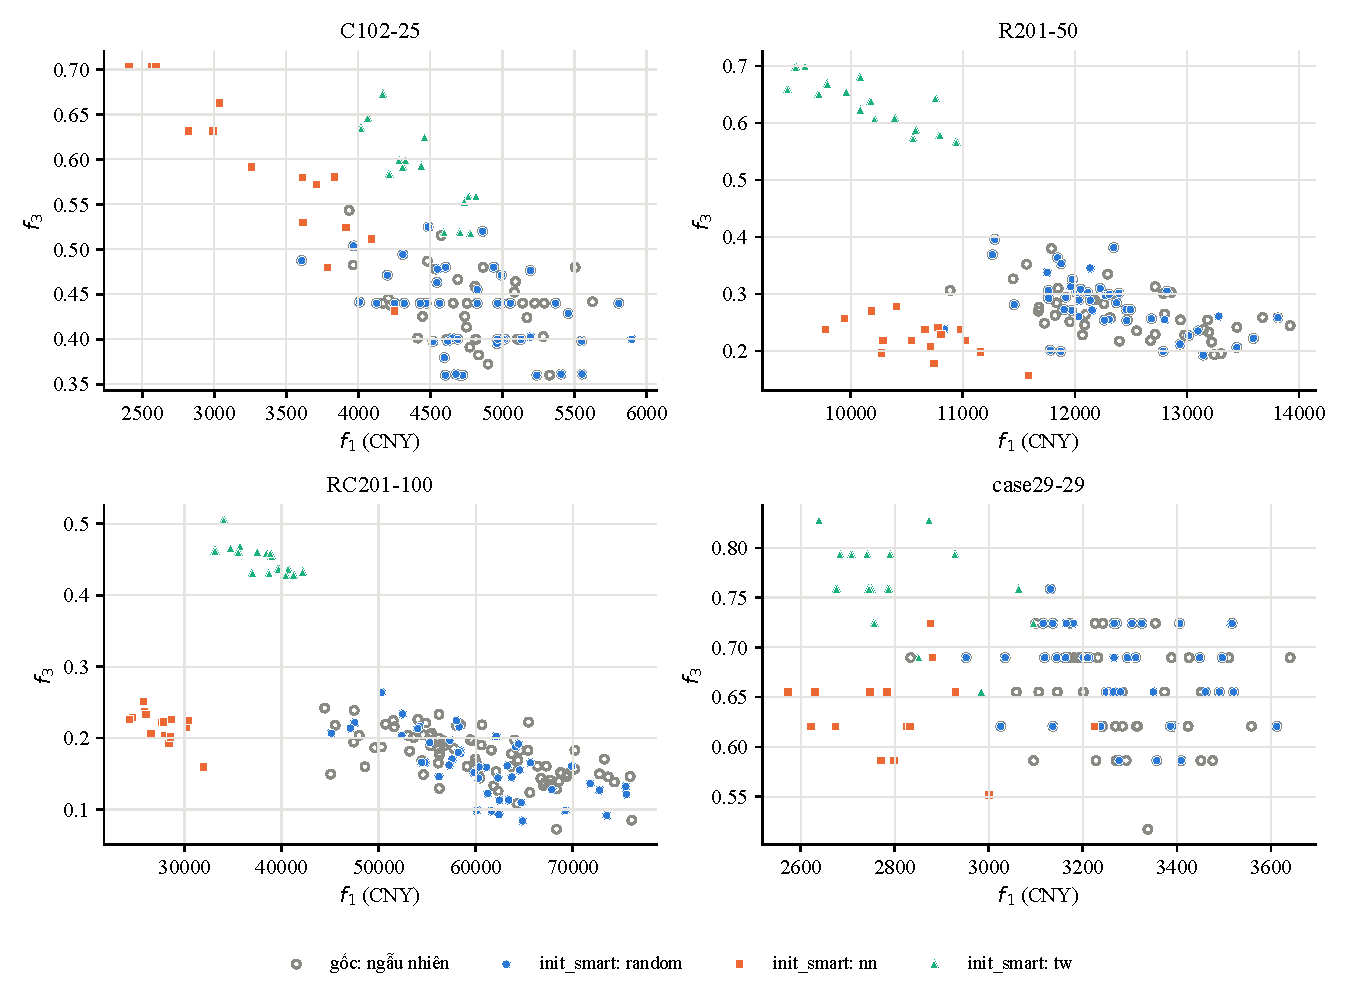
\includegraphics[width=\textwidth]{quan_the_dau.pdf}
\caption{Quần thể ban đầu với seed 0 trên mặt phẳng $f_1$--$f_3$: thuật toán gốc (vòng tròn rỗng) và
\code{init\_smart} theo từng nguồn}
\label{fig:init}
\end{figure}

\subsection{Kết quả cuối}

Ở cùng 200 thế hệ và cùng 16.080 lần đánh giá, \code{init\_smart} cho HV cao hơn hẳn thuật toán gốc trên
cả bốn instance với $p < 0{,}001$ (bảng~\ref{tab:main-c102} đến~\ref{tab:main-case29}): C102-25 từ 0,663
lên 1,099; R201-50 từ 0,385 lên 0,687; RC201-100 từ 0,328 lên 0,877; case29-29 từ 0,550 lên 0,775. IGD
giảm tương ứng và độ lệch chuẩn của HV nhỏ hơn, tức kết quả ổn định hơn giữa các seed. Cải tiến này
không tốn thêm lần đánh giá nào và thời gian chạy gần như không đổi.

So với thuật toán gốc được chạy dài hơn 3,3 đến 6,8 lần số lần đánh giá, \code{init\_smart} 200 thế hệ
vẫn tốt hơn trên C102-25 (1,099 so với 0,911, $p = 0{,}034$) nhưng kém hơn trên ba instance còn lại
($p$ từ 0,0007 đến 0,028). Như vậy khởi tạo thông minh chủ yếu giúp thuật toán tới vùng tốt nhanh hơn;
khi được chạy đủ lâu, thuật toán gốc vẫn bắt kịp và vượt.

\section{Hiệu quả của tìm kiếm cục bộ}

\subsection{Bảng kết quả}

\begin{table}[H]
\centering
\caption{Kết quả trên C102-25 (10 seed; $G$ là số thế hệ; $p$ so với Gốc 200 thế hệ)}
\label{tab:main-c102}
\resizebox{\textwidth}{!}{\begin{tabular}{@{}lrllrrrrr@{}}
\toprule
Cấu hình & $G$ & HV & IGD & SP & Số điểm & Số lần đánh giá & Thời gian (s) & $p$ \\
\midrule
Gốc & 200 & 0{,}663 $\pm$ 0{,}248 & 0{,}366 $\pm$ 0{,}112 & 0{,}072 & 9{,}7 & 16.080 & 6{,}3 & -- \\
Gốc, cùng số lần đánh giá & 670 & 0{,}911 $\pm$ 0{,}208 & 0{,}274 $\pm$ 0{,}045 & 0{,}037 & 21{,}1 & 53.680 & 18{,}9 & 0{,}019 \\
init\_smart & 200 & 1{,}099 $\pm$ 0{,}097 & 0{,}239 $\pm$ 0{,}028 & 0{,}045 & 16{,}7 & 16.080 & 5{,}1 & $<$0{,}001 \\
LS (reject) & 200 & 0{,}596 $\pm$ 0{,}229 & 0{,}396 $\pm$ 0{,}178 & 0{,}044 & 15{,}3 & 65.719 & 23{,}8 & 0{,}705 \\
LS (evaluate\_actual) & 200 & 0{,}691 $\pm$ 0{,}137 & 0{,}346 $\pm$ 0{,}074 & 0{,}089 & 13{,}8 & 56.704 & 20{,}9 & 0{,}545 \\
init + LS (reject) & 200 & 1{,}177 $\pm$ 0{,}076 & 0{,}235 $\pm$ 0{,}064 & 0{,}103 & 6{,}3 & 57.251 & 19{,}8 & $<$0{,}001 \\
init + LS (evaluate\_actual) & 200 & \textbf{1{,}193 $\pm$ 0{,}067} & \textbf{0{,}210 $\pm$ 0{,}018} & 0{,}098 & 6{,}9 & 53.661 & 19{,}1 & $<$0{,}001 \\
\bottomrule
\end{tabular}
}
\end{table}

\begin{table}[H]
\centering
\caption{Kết quả trên R201-50}
\label{tab:main-r201}
\resizebox{\textwidth}{!}{\begin{tabular}{@{}lrllrrrrr@{}}
\toprule
Cấu hình & $G$ & HV & IGD & SP & Số điểm & Số lần đánh giá & Thời gian (s) & $p$ \\
\midrule
Gốc & 200 & 0{,}385 $\pm$ 0{,}080 & 0{,}448 $\pm$ 0{,}083 & 0{,}030 & 19{,}7 & 16.080 & 10{,}8 & -- \\
Gốc, cùng số lần đánh giá & 1016 & \textbf{0{,}898 $\pm$ 0{,}107} & \textbf{0{,}110 $\pm$ 0{,}048} & 0{,}012 & 48{,}3 & 81.360 & 47{,}0 & $<$0{,}001 \\
init\_smart & 200 & 0{,}687 $\pm$ 0{,}074 & 0{,}212 $\pm$ 0{,}047 & 0{,}026 & 25{,}9 & 16.080 & 10{,}7 & $<$0{,}001 \\
LS (reject) & 200 & 0{,}420 $\pm$ 0{,}105 & 0{,}414 $\pm$ 0{,}108 & 0{,}022 & 33{,}3 & 113.295 & 71{,}1 & 0{,}545 \\
LS (evaluate\_actual) & 200 & 0{,}505 $\pm$ 0{,}108 & 0{,}357 $\pm$ 0{,}094 & 0{,}015 & 49{,}8 & 85.998 & 53{,}3 & 0{,}016 \\
init + LS (reject) & 200 & 0{,}778 $\pm$ 0{,}110 & 0{,}164 $\pm$ 0{,}059 & 0{,}015 & 44{,}4 & 102.187 & 60{,}4 & $<$0{,}001 \\
init + LS (evaluate\_actual) & 200 & 0{,}812 $\pm$ 0{,}112 & 0{,}145 $\pm$ 0{,}065 & 0{,}021 & 47{,}6 & 81.349 & 48{,}9 & $<$0{,}001 \\
\bottomrule
\end{tabular}
}
\end{table}

\begin{table}[H]
\centering
\caption{Kết quả trên RC201-100}
\label{tab:main-rc201}
\resizebox{\textwidth}{!}{\begin{tabular}{@{}lrllrrrrr@{}}
\toprule
Cấu hình & $G$ & HV & IGD & SP & Số điểm & Số lần đánh giá & Thời gian (s) & $p$ \\
\midrule
Gốc & 200 & 0{,}328 $\pm$ 0{,}048 & 0{,}633 $\pm$ 0{,}083 & 0{,}024 & 26{,}4 & 16.080 & 20{,}9 & -- \\
Gốc, cùng số lần đánh giá & 1374 & 1{,}001 $\pm$ 0{,}109 & 0{,}127 $\pm$ 0{,}060 & 0{,}009 & 50{,}9 & 110.000 & 109{,}6 & $<$0{,}001 \\
init\_smart & 200 & 0{,}877 $\pm$ 0{,}103 & 0{,}173 $\pm$ 0{,}064 & 0{,}015 & 24{,}5 & 16.080 & 20{,}1 & $<$0{,}001 \\
LS (reject) & 200 & 0{,}377 $\pm$ 0{,}076 & 0{,}570 $\pm$ 0{,}072 & 0{,}017 & 26{,}2 & 127.027 & 148{,}9 & 0{,}151 \\
LS (evaluate\_actual) & 200 & 0{,}544 $\pm$ 0{,}079 & 0{,}425 $\pm$ 0{,}069 & 0{,}013 & 33{,}6 & 93.088 & 111{,}1 & $<$0{,}001 \\
init + LS (reject) & 200 & 0{,}944 $\pm$ 0{,}136 & 0{,}147 $\pm$ 0{,}070 & 0{,}009 & 51{,}3 & 130.477 & 151{,}5 & $<$0{,}001 \\
init + LS (evaluate\_actual) & 200 & \textbf{1{,}080 $\pm$ 0{,}059} & \textbf{0{,}075 $\pm$ 0{,}026} & 0{,}007 & 51{,}9 & 109.971 & 127{,}3 & $<$0{,}001 \\
\bottomrule
\end{tabular}
}
\end{table}

\begin{table}[H]
\centering
\caption{Kết quả trên case29-29}
\label{tab:main-case29}
\resizebox{\textwidth}{!}{\begin{tabular}{@{}lrllrrrrr@{}}
\toprule
Cấu hình & $G$ & HV & IGD & SP & Số điểm & Số lần đánh giá & Thời gian (s) & $p$ \\
\midrule
Gốc & 200 & 0{,}550 $\pm$ 0{,}123 & 0{,}349 $\pm$ 0{,}089 & 0{,}090 & 9{,}3 & 16.080 & 8{,}0 & -- \\
Gốc, cùng số lần đánh giá & 1030 & \textbf{0{,}874 $\pm$ 0{,}106} & \textbf{0{,}161 $\pm$ 0{,}032} & 0{,}054 & 16{,}1 & 82.480 & 34{,}7 & $<$0{,}001 \\
init\_smart & 200 & 0{,}775 $\pm$ 0{,}075 & 0{,}175 $\pm$ 0{,}048 & 0{,}061 & 14{,}3 & 16.080 & 7{,}8 & $<$0{,}001 \\
LS (reject) & 200 & 0{,}612 $\pm$ 0{,}128 & 0{,}308 $\pm$ 0{,}085 & 0{,}035 & 15{,}7 & 89.059 & 37{,}6 & 0{,}364 \\
LS (evaluate\_actual) & 200 & 0{,}697 $\pm$ 0{,}092 & 0{,}249 $\pm$ 0{,}075 & 0{,}053 & 15{,}6 & 81.316 & 34{,}0 & 0{,}008 \\
init + LS (reject) & 200 & 0{,}765 $\pm$ 0{,}070 & 0{,}186 $\pm$ 0{,}036 & 0{,}068 & 16{,}5 & 88.581 & 37{,}5 & 0{,}001 \\
init + LS (evaluate\_actual) & 200 & 0{,}803 $\pm$ 0{,}054 & 0{,}175 $\pm$ 0{,}039 & 0{,}036 & 19{,}6 & 82.445 & 37{,}0 & $<$0{,}001 \\
\bottomrule
\end{tabular}
}
\end{table}

\subsection{Tìm kiếm cục bộ đứng riêng}

Với chính sách \code{reject}, tìm kiếm cục bộ đứng riêng không tạo khác biệt có ý nghĩa thống kê so với
thuật toán gốc trên instance nào ($p$ từ 0,151 đến 0,705), dù dùng gấp 4,1 đến 7,9 lần số lần đánh giá.
Với \code{evaluate\_actual}, HV tăng có ý nghĩa trên R201-50 ($p = 0{,}016$), RC201-100 ($p < 0{,}001$) và
case29-29 ($p = 0{,}008$), không có ý nghĩa trên C102-25. Trên RC201-100, \code{evaluate\_actual} tốt
hơn \code{reject} rõ rệt (HV 0,544 so với 0,377, $p = 0{,}0009$; front của nó phủ trung bình 96\% front
của \code{reject} theo SC).

\subsection{Thống kê bên trong tìm kiếm cục bộ}
\label{sec:ls-stats}

\begin{table}[H]
\centering
\caption{Thống kê tìm kiếm cục bộ (trung bình một lần chạy 200 thế hệ; tỉ lệ tính trên số ứng viên)}
\label{tab:lsstats}
\resizebox{\textwidth}{!}{\begin{tabular}{@{}llrrrrrrr@{}}
\toprule
Instance & Cấu hình & Số lần chạy & Ứng viên & Nhận (\%) & Lệch biên (\%) & Loại do lệch (\%) & Loại do số xe (\%) & Thời gian LS (\%) \\
\midrule
C102-25 & LS (reject) & 3.188 & 58.757 & 3{,}5 & 85{,}2 & 85{,}2 & 0{,}0 & 76 \\
 & LS (evaluate\_actual) & 3.188 & 45.134 & 6{,}9 & 85{,}7 & 0{,}0 & 0{,}0 & 72 \\
 & init + LS (reject) & 3.187 & 45.580 & 2{,}7 & 88{,}3 & 88{,}3 & 0{,}0 & 72 \\
 & init + LS (evaluate\_actual) & 3.211 & 40.166 & 5{,}4 & 88{,}3 & 0{,}0 & 0{,}0 & 71 \\
\midrule
R201-50 & LS (reject) & 3.171 & 113.048 & 3{,}5 & 75{,}4 & 75{,}4 & 0{,}0 & 87 \\
 & LS (evaluate\_actual) & 3.218 & 77.156 & 7{,}7 & 72{,}4 & 0{,}0 & 0{,}0 & 83 \\
 & init + LS (reject) & 3.200 & 95.922 & 4{,}3 & 73{,}0 & 73{,}0 & 0{,}0 & 85 \\
 & init + LS (evaluate\_actual) & 3.222 & 69.374 & 7{,}5 & 73{,}5 & 0{,}0 & 0{,}0 & 82 \\
\midrule
RC201-100 & LS (reject) & 3.176 & 125.536 & 4{,}5 & 77{,}9 & 77{,}9 & 0{,}0 & 89 \\
 & LS (evaluate\_actual) & 3.178 & 84.103 & 9{,}4 & 75{,}1 & 0{,}0 & 1{,}0 & 85 \\
 & init + LS (reject) & 3.191 & 125.967 & 4{,}3 & 69{,}6 & 69{,}6 & 0{,}0 & 89 \\
 & init + LS (evaluate\_actual) & 3.189 & 99.652 & 7{,}1 & 68{,}3 & 0{,}0 & 0{,}1 & 87 \\
\midrule
case29-29 & LS (reject) & 3.200 & 96.764 & 8{,}7 & 16{,}8 & 16{,}8 & 0{,}0 & 82 \\
 & LS (evaluate\_actual) & 3.182 & 85.424 & 9{,}9 & 16{,}0 & 0{,}0 & 0{,}0 & 81 \\
 & init + LS (reject) & 3.185 & 101.040 & 7{,}4 & 15{,}4 & 15{,}4 & 0{,}0 & 82 \\
 & init + LS (evaluate\_actual) & 3.188 & 91.575 & 8{,}2 & 12{,}8 & 0{,}0 & 0{,}0 & 81 \\

\bottomrule
\end{tabular}
}
\end{table}

Bảng~\ref{tab:lsstats} giải thích kết quả trên. Mỗi lần chạy có khoảng 3.200 lần tìm kiếm cục bộ được
kích hoạt, đúng với kỳ vọng $p_{ls} \cdot N_{pop} \cdot G = 0{,}2 \cdot 80 \cdot 200 = 3.200$. Trên ba
instance Solomon, 68 đến 88\% ứng viên bị lệch biên tuyến. Với chính sách \code{reject}, toàn bộ số ứng
viên đó bị loại và chỉ 2,7 đến 4,5\% ứng viên được nhận: phần lớn ngân sách đánh giá bị tiêu vào các
bước không bao giờ được dùng. Với \code{evaluate\_actual}, tỉ lệ nhận tăng khoảng gấp đôi (5,4 đến 9,9\%)
và cùng ngân sách đổi được nhiều cải thiện hơn. Trên case29, tỉ lệ lệch biên chỉ 13 đến 17\%: dữ liệu này
có tải trọng 4000 kg, chưa giới hạn số xe và khung thời gian rộng, nên chỗ cắt tuyến ít nhạy với thứ tự
khách bên trong một tuyến.

Chính sách số xe gần như không phải can thiệp: chỉ trên RC201-100 với \code{evaluate\_actual} có khoảng
1\% ứng viên bị loại vì làm tăng số xe vượt giới hạn. Cột cuối cho thấy tìm kiếm cục bộ chiếm 71 đến 89\%
thời gian chạy, nên đây là phần tốn kém nhất của thuật toán khi bật cải tiến này.

\subsection{Kết hợp hai cải tiến}

Cấu hình init + LS (evaluate\_actual) cho HV cao nhất trong các cấu hình 200 thế hệ trên cả bốn instance.
So với chỉ bật \code{init\_smart}, phần tìm kiếm cục bộ thêm vào làm HV tăng có ý nghĩa trên C102-25
($p = 0{,}019$), R201-50 ($p = 0{,}016$) và RC201-100 ($p = 0{,}0004$), không có ý nghĩa trên case29-29
($p = 0{,}36$). Trên RC201-100, chính sách \code{evaluate\_actual} cũng tốt hơn \code{reject} khi đã có
khởi tạo thông minh (HV 1,080 so với 0,944, $p = 0{,}019$).

\subsection{So sánh ở cùng số lần đánh giá}

Đây là phép so công bằng nhất cho tìm kiếm cục bộ. So init + LS (evaluate\_actual) với thuật toán gốc chạy
đủ lâu để có cùng số lần đánh giá:
\begin{itemize}
  \item C102-25: cấu hình kết hợp tốt hơn rõ (HV 1,193 so với 0,911, $p = 0{,}0005$; front của nó phủ
        trung bình 86\% front của thuật toán gốc, chiều ngược lại chỉ 4\%);
  \item RC201-100: cấu hình kết hợp tốt hơn (HV 1,080 so với 1,001, $p = 0{,}034$);
  \item R201-50 và case29-29: thuật toán gốc chạy dài có HV cao hơn (0,898 so với 0,812 và 0,874 so với
        0,803), nhưng khác biệt chưa có ý nghĩa thống kê ($p = 0{,}096$ ở cả hai).
\end{itemize}
Mọi cấu hình chỉ có tìm kiếm cục bộ (không có khởi tạo thông minh) đều kém thuật toán gốc chạy dài. Kết
luận là trong cấu hình hiện tại, tìm kiếm cục bộ chỉ đáng dùng khi đi kèm khởi tạo thông minh, và lợi
ích phụ thuộc instance.

\section{Hội tụ, phân bố kết quả và mặt Pareto}

\begin{figure}[H]
\centering
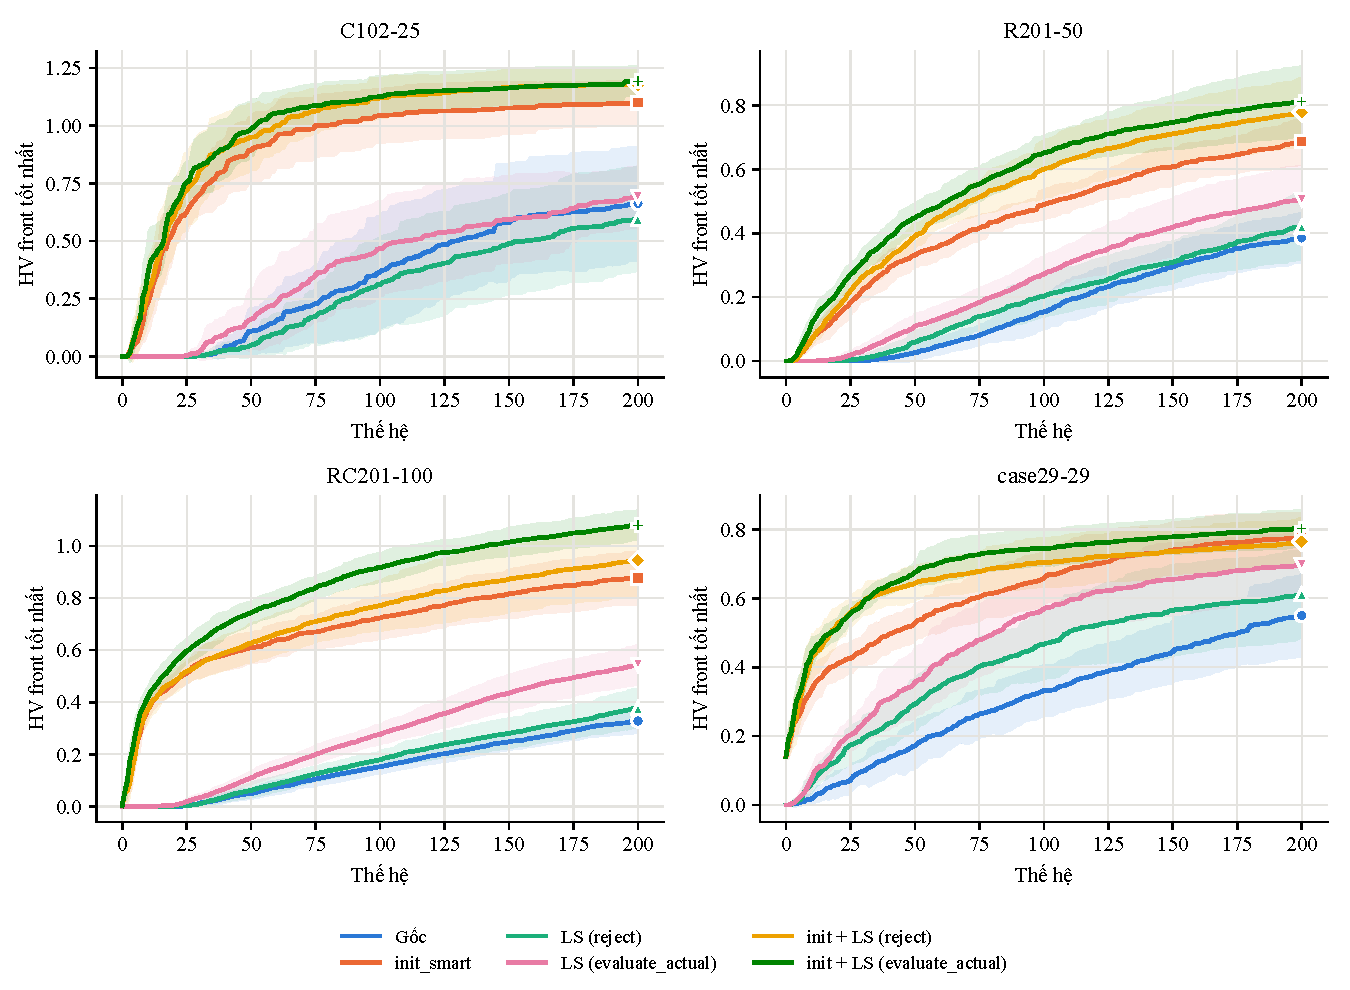
\includegraphics[width=\textwidth]{hoi_tu_hv.pdf}
\caption{HV của front tốt nhất theo thế hệ, trung bình $\pm$ độ lệch chuẩn qua 10 seed}
\label{fig:hoitu}
\end{figure}

Hình~\ref{fig:hoitu} cho thấy hai nhóm đường tách bạch. Các cấu hình có \code{init\_smart} có HV dương
ngay từ những thế hệ đầu và tăng nhanh trong khoảng 25 thế hệ đầu. Trên ba instance Solomon, các cấu
hình bắt đầu từ quần thể ngẫu nhiên có HV trung bình bằng 0 trong 10 đến 28 thế hệ đầu, vì front lúc đó
nằm ngoài vùng chuẩn hoá chung (điều này đã được ghi trong README của nhóm và là bình thường); trên
case29-29, HV dương ngay từ thế hệ thứ nhất. Ở mọi instance, HV vẫn còn tăng ở thế hệ 200, tức
200 thế hệ chưa đủ để thuật toán hội tụ hẳn.

\begin{figure}[H]
\centering
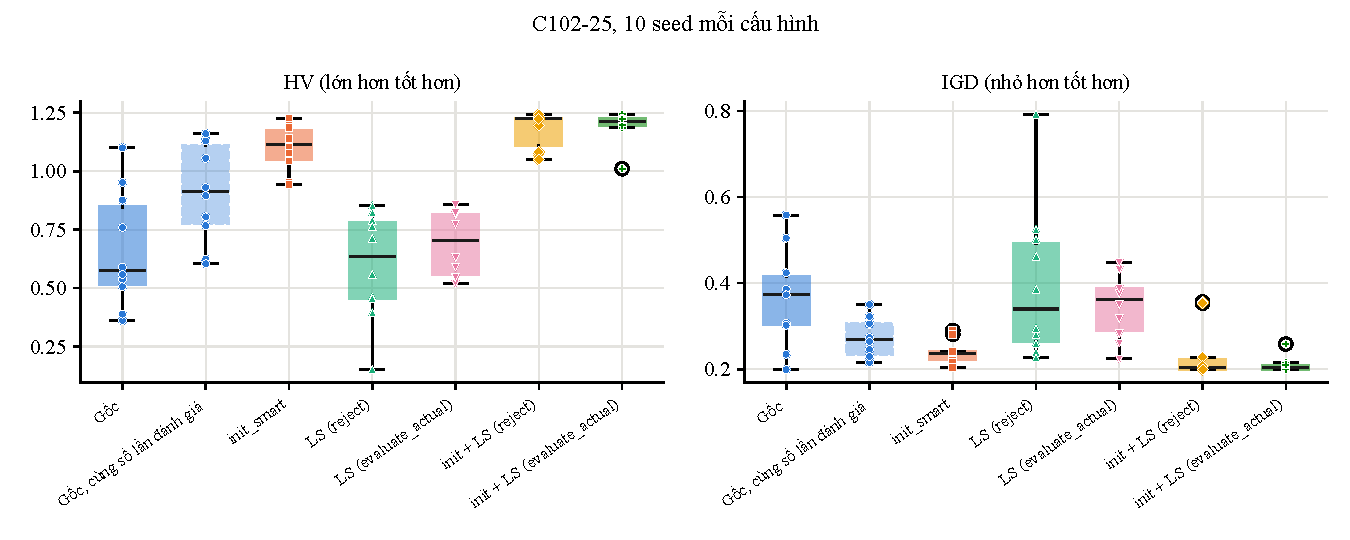
\includegraphics[width=\textwidth]{box_C102-25.pdf}\\[2pt]
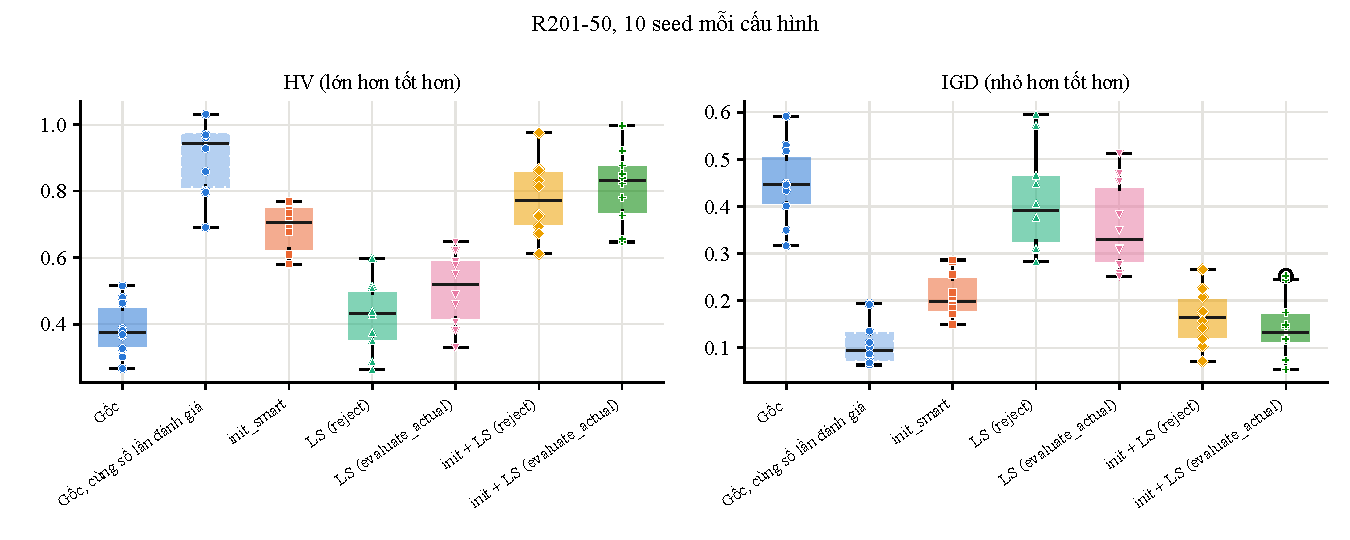
\includegraphics[width=\textwidth]{box_R201-50.pdf}
\caption{Phân bố HV và IGD qua 10 seed trên C102-25 và R201-50}
\label{fig:box1}
\end{figure}

\begin{figure}[H]
\centering
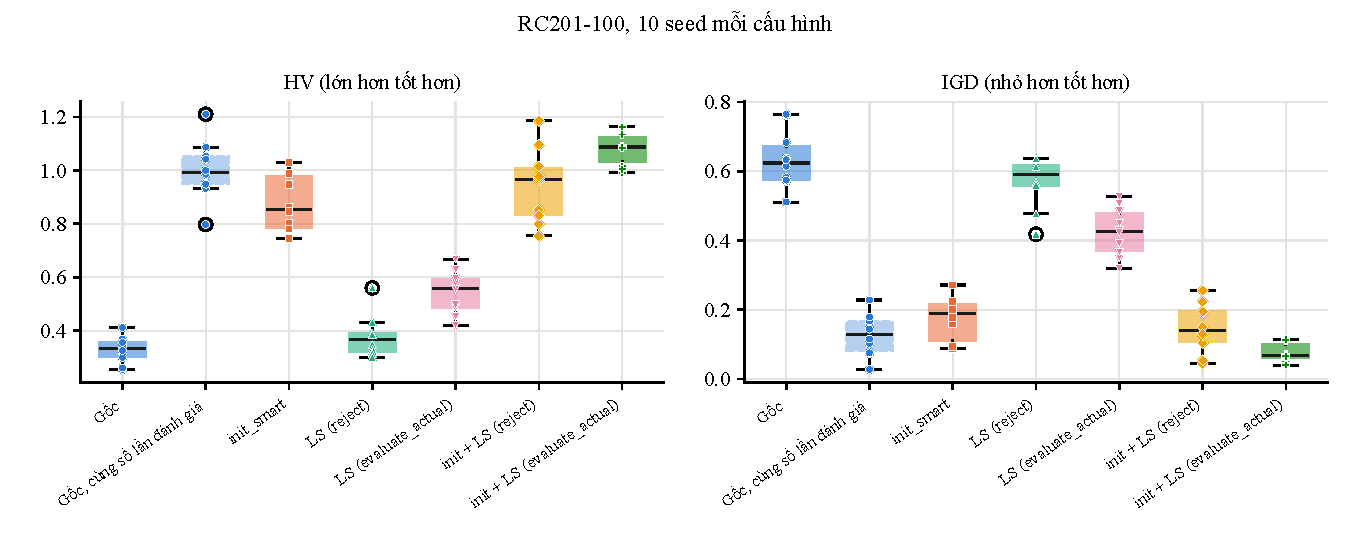
\includegraphics[width=\textwidth]{box_RC201-100.pdf}\\[2pt]
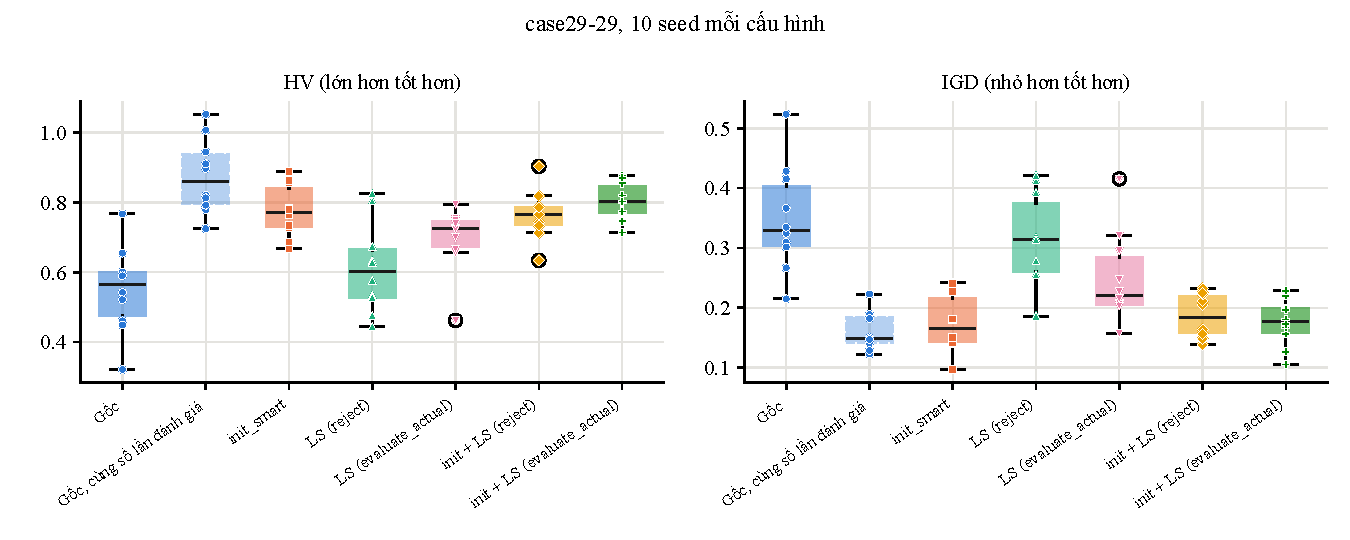
\includegraphics[width=\textwidth]{box_case29-29.pdf}
\caption{Phân bố HV và IGD qua 10 seed trên RC201-100 và case29-29}
\label{fig:box2}
\end{figure}

Biểu đồ hộp ở hình~\ref{fig:box1} và~\ref{fig:box2} xác nhận các nhận xét ở trên: hộp của các cấu hình có
\code{init\_smart} nằm cao hơn và hẹp hơn hộp của thuật toán gốc 200 thế hệ; hộp của thuật toán gốc chạy
dài (viền nét đứt) nằm cùng mức với các cấu hình kết hợp trên R201-50 và case29-29.

\begin{figure}[H]
\centering
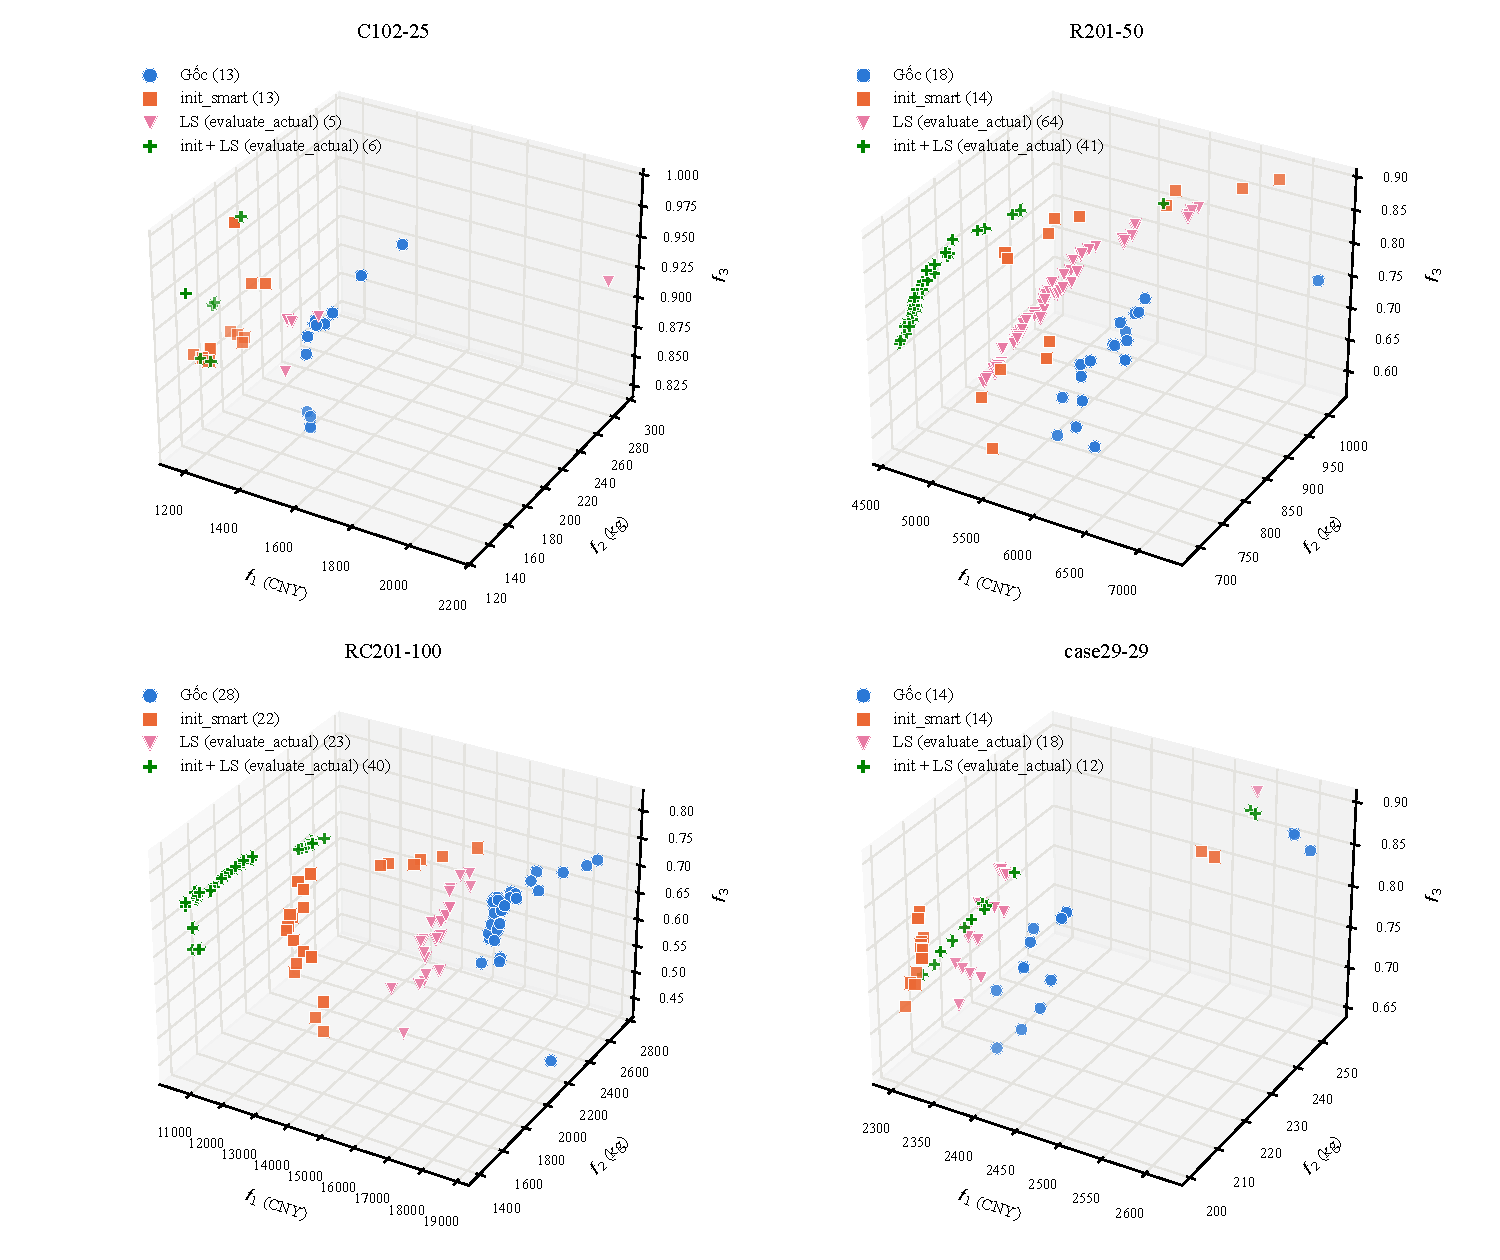
\includegraphics[width=\textwidth]{pareto_3d.pdf}
\caption{Front cuối không bị trội với seed 0, đơn vị gốc ($f_1$, $f_2$ cực tiểu, $f_3$ cực đại; số trong
ngoặc là số điểm trên front)}
\label{fig:pareto}
\end{figure}

Hình~\ref{fig:pareto} vẽ front cuối của bốn cấu hình với seed 0. Front của các cấu hình có khởi tạo thông
minh nằm ở vùng chi phí và khí thải thấp hơn hẳn, nhất là trên RC201-100. Hệ số tương quan Pearson giữa
$f_1$ và $f_2$ trên front gộp 10 seed dao động từ $-0{,}03$ đến 0,96 tuỳ cấu hình và instance. Tương quan
cao khi $f_1$ chủ yếu đi theo quãng đường, vì $f_2$ tỉ lệ với quãng đường; tương quan thấp khi phần phạt
đến muộn $F_4$ chi phối $f_1$, đúng như nhóm đã nhận xét ở giai đoạn 1 với các instance 100 khách.

Về ràng buộc số xe, front cuối của mọi cấu hình, mọi seed trên cả bốn instance đều không vượt giới hạn số
xe. Trội có ràng buộc của thuật toán gốc loại các nghiệm vượt giới hạn, và tìm kiếm cục bộ không làm nghiệm
hợp lệ trở thành không hợp lệ.

\section{Thảo luận}

\paragraph{Khởi tạo thông minh.} Đây là cải tiến có lợi rõ nhất: tốt hơn thuật toán gốc ở cả bốn instance,
không tốn thêm lần đánh giá, kết quả ổn định hơn giữa các seed. Hai heuristic bổ sung cho nhau: NN gieo
điểm ở vùng chi phí thấp, TW gieo điểm ở vùng hài lòng cao. Hạn chế là lợi thế giảm dần khi thuật toán
được chạy lâu hơn.

\paragraph{Tìm kiếm cục bộ.} Cách cắt tuyến \code{capacity\_time} làm phần lớn bước đi trong một tuyến bị
lệch biên, nên phiên bản thuần trong tuyến (\code{reject}) lãng phí phần lớn ngân sách đánh giá và không
hiệu quả. Cho phép đánh giá bằng bộ tuyến thật (\code{evaluate\_actual}) khắc phục được một phần và đem
lại cải thiện có ý nghĩa trên các instance lớn. Tuy vậy, ở cùng số lần đánh giá, tìm kiếm cục bộ chỉ thắng
thuật toán gốc chạy dài khi đi cùng khởi tạo thông minh, và chỉ trên hai trong bốn instance.

\paragraph{Giới hạn của thực nghiệm.} Thực nghiệm dùng bốn instance và 10 seed; kết luận chưa được kiểm
chứng trên đủ chín instance Solomon của bài báo. Kiểm định rank-sum được thực hiện riêng cho từng cặp,
không hiệu chỉnh cho nhiều phép so sánh. Các seed được ghép cặp giữa các cấu hình nên kiểm định có dấu
hạng (signed-rank) có thể phù hợp hơn; việc chọn kiểm định chính thức thuộc phần việc của TV3.

\chapter{TIẾN ĐỘ, ĐÁNH GIÁ VÀ HƯỚNG HOÀN THIỆN}
\label{chap:tiendo}

\section{Tiến độ thực hiện}

Bảng~\ref{tab:tiendo} đối chiếu kế hoạch trong README của nhóm với thời điểm thực hiện, lấy theo lịch sử
commit trên nhánh \code{feat/tv2-init-local-search}.

\begin{table}[H]
\centering
\caption{Tiến độ phần việc TV2}
\label{tab:tiendo}
\begin{tabularx}{\textwidth}{@{}p{3.3cm}Xp{2.2cm}@{}}
\toprule
\textbf{Giai đoạn (kế hoạch)} & \textbf{Công việc} & \textbf{Thực hiện} \\
\midrule
Giai đoạn 2 \newline (12/11--18/11) &
  Khảo sát mã nguồn; cài đặt \code{init\_smart}, \code{local\_search}, lớp dán \code{tv2\_hooks};
  170 test đơn vị; harness NSGA-II tạm vì \code{nsga2.py} lúc đó chưa có; mốc hồi quy khi tắt cờ;
  thí nghiệm sơ bộ trên harness; tài liệu hợp đồng giao diện & 12/11 \\
\midrule
Giai đoạn 3 \newline (19/11--25/11) &
  Quy trình ghép nhánh và xử lý xung đột \code{config.yaml}; ghép thử với nhánh của TV4 trong một nhánh
  tạm và kiểm tra tìm kiếm cục bộ chạy cùng DP split & 12/11 \\
 & Ghép nhánh chính mới nhất (đã có \code{nsga2.py} của TV1, cải tiến của TV3 và TV4) vào nhánh TV2;
  gắn hai cải tiến vào \code{nsga2.py} thật; thêm test tích hợp; 432 test pass & 27/11 \\
\midrule
Giai đoạn 4 \newline (26/11--02/12) &
  Chạy lại toàn bộ thực nghiệm trên thuật toán thật (440 lần chạy); sinh bảng và hình tự động; viết
  báo cáo này & 27/11 \\
\bottomrule
\end{tabularx}
\end{table}

Phần việc của giai đoạn 2 hoàn thành sớm. Phần gắn vào thuật toán thật bị chậm so với kế hoạch: thuật
toán gốc của TV1 được ghép vào nhánh chính ngày 13/11, nhưng nhánh TV2 chỉ cập nhật nhánh chính vào ngày
27/11, khi nhóm trưởng đã ghép xong các nhánh của TV3 và TV4. Trong khoảng thời gian đó, thực nghiệm của
TV2 chạy trên harness tạm; các số liệu trong báo cáo này đều đã được chạy lại trên thuật toán thật. Việc
ghép bốn nhánh vào nhánh chính ở giai đoạn 3 do nhóm trưởng thực hiện; TV2 chuẩn bị quy trình, mốc hồi
quy và kiểm tra tương thích.

\section{Đối chiếu với yêu cầu}

\begin{longtable}{@{}p{8.4cm}p{1.8cm}p{4.3cm}@{}}
\caption{Đối chiếu kết quả với các yêu cầu của phần việc TV2}\label{tab:doichieu}\\
\toprule
\textbf{Yêu cầu} & \textbf{Trạng thái} & \textbf{Bằng chứng} \\
\midrule
\endfirsthead
\toprule
\textbf{Yêu cầu} & \textbf{Trạng thái} & \textbf{Bằng chứng} \\
\midrule
\endhead
Khởi tạo trộn NN, theo khung giờ và ngẫu nhiên theo tỉ lệ trong cấu hình & Đạt & Chương~\ref{chap:init} \\
Hai thứ tự tất định có biến thể, quần thể không trùng lặp & Đạt & mục 3.4, 3.5; test \\
Mọi cá thể là hoán vị hợp lệ; tỉ lệ các nhóm đúng & Đạt & 91 test của \code{init\_smart} \\
2-opt và Or-opt trong từng tuyến sau đột biến & Đạt & Chương~\ref{chap:ls} \\
Định nghĩa rõ thế nào là tốt hơn khi có ba mục tiêu & Đạt & mục 4.4: Pareto hoặc tổng có trọng số \\
Giới hạn số vòng lặp của tìm kiếm cục bộ & Đạt & ba trần cứng, có test \\
Kiểm tra việc cắt lại tuyến sau khi ghép (lệch biên) & Đạt & mục~\ref{sec:drift}; phản ví dụ trong test \\
Mỗi tuyến giữ nguyên tập khách; không bước nào làm tuyến tệ hơn theo tiêu chí & Đạt & test \\
Tham số trong \code{config.yaml}, cờ mặc định tắt & Đạt & mục 3.1, 4.1 \\
Cờ tắt không dùng bộ sinh ngẫu nhiên; ra đúng thuật toán gốc & Đạt & mục~\ref{sec:regress}: trùng từng bit \\
Mọi lần đánh giá thêm được đếm vào \code{n\_evals} & Đạt & công thức~\ref{eq:nevals}, có test \\
Chạy 10 seed trên ít nhất 3 instance, so HV với thuật toán gốc & Đạt & Chương~\ref{chap:thucnghiem}: 4 instance \\
So sánh cùng số lần đánh giá & Đạt & cấu hình gốc chạy dài \\
Chuẩn bị mốc hồi quy và quy trình ghép nhánh & Đạt & \code{tv2\_merge\_playbook.md} \\
Biểu đồ front Pareto 3D, hội tụ HV, hộp HV và IGD & Đạt & hình~\ref{fig:hoitu}--\ref{fig:pareto} \\
Ghép bốn nhánh vào nhánh chính & Nhóm trưởng thực hiện & lịch sử nhánh chính 27/11 \\
Kiểm định thống kê chính thức cho toàn bộ ablation & Chưa & thuộc phần việc TV3 \\
\bottomrule
\end{longtable}

\section{Đánh giá}

\paragraph{Điểm làm được.} Hai cải tiến chạy được trên thuật toán thật, đúng các quy tắc chung của nhóm, có
bộ test bao phủ các trường hợp biên và một bằng chứng mạnh rằng nhánh cờ tắt không đổi kết quả: trùng từng
bit với mốc do TV4 sinh từ mã chưa sửa. Thực nghiệm có tách seed tinh chỉnh khỏi seed báo cáo và có phép so
ở cùng số lần đánh giá, nên kết luận không bị thiên vị cho tìm kiếm cục bộ. Khởi tạo thông minh cho cải
thiện rõ và ổn định trên cả bốn instance.

\paragraph{Điểm còn hạn chế.}
\begin{itemize}
  \item Tìm kiếm cục bộ tốn nhiều lần đánh giá (gấp 3,3 đến 8,1 lần thuật toán gốc) và chiếm 71 đến 89\%
        thời gian chạy. Ở cùng số lần đánh giá, nó chỉ có lợi khi đi cùng khởi tạo thông minh và chỉ trên
        hai trong bốn instance.
  \item Với chính sách mặc định \code{reject}, phần lớn ứng viên bị loại vì lệch biên tuyến, nên tìm kiếm
        cục bộ thuần trong tuyến gần như không có tác dụng với cách cắt \code{capacity\_time}.
  \item Mỗi ứng viên được chấm lại bằng toàn bộ bộ giải mã, $O(n)$, dù chỉ một tuyến thay đổi.
  \item Thực nghiệm mới trên bốn instance, chưa đủ chín instance Solomon của bài báo.
  \item Lợi thế của khởi tạo thông minh giảm khi thuật toán được chạy lâu hơn.
\end{itemize}

\section{Hướng hoàn thiện và cải tiến}

\begin{enumerate}
  \item \textbf{Chọn chính sách lệch biên mặc định.} Số liệu cho thấy \code{evaluate\_actual} tốt hơn
        \code{reject} trên các instance lớn và chưa kém ở đâu có ý nghĩa thống kê. Nên đề xuất với TV4 (người
        phụ trách tinh chỉnh) đổi mặc định sau khi chạy đủ chín instance.
  \item \textbf{Đánh giá tăng dần.} Thay vì giải mã lại cả hoán vị, chỉ tính lại tuyến bị thay đổi và kiểm
        tra chỗ cắt ở hai đầu tuyến. Giờ đến trên các tuyến khác không phụ thuộc tuyến này, vì mỗi xe xuất
        phát độc lập từ kho, nên phần tiết kiệm có thể lớn với $n = 100$.
  \item \textbf{Bước đi giữa các tuyến.} Thêm relocate, swap và 2-opt* giữa hai tuyến. Với cách cắt theo
        thời gian, chuyển khách giữa các tuyến có thể hợp với cấu trúc bài toán hơn bước đi trong tuyến.
  \item \textbf{Chọn cá thể để tìm kiếm cục bộ.} Chỉ áp dụng cho con thuộc front tốt nhất, hoặc giảm $p_{ls}$
        theo thời gian, để giảm số lần đánh giá ở các thế hệ đầu khi quần thể còn kém.
  \item \textbf{Khởi tạo đa dạng hơn.} Dùng láng giềng gần nhất ngẫu nhiên hoá (chọn trong $k$ khách gần
        nhất) hoặc heuristic chèn có xét khung thời gian kiểu Solomon I1 thay cho phép hoán đổi ngẫu nhiên.
  \item \textbf{Thực nghiệm đầy đủ.} Chạy trên chín instance Solomon và case29, so cả theo thời gian chạy,
        và để TV3 áp dụng kiểm định có hiệu chỉnh cho nhiều phép so sánh.
\end{enumerate}

\chapter*{KẾT LUẬN}
\addcontentsline{toc}{chapter}{Kết luận}

Phần việc TV2 đã hoàn thành hai cải tiến cho thuật toán NSGA-II giải bài toán MOGVRPTW của nhóm. Khởi tạo
thông minh tạo quần thể ban đầu từ thứ tự láng giềng gần nhất, thứ tự theo khung giờ và hoán vị ngẫu
nhiên theo tỉ lệ cấu hình, có biến thể và khử trùng. Tìm kiếm cục bộ cải thiện từng con bằng 2-opt và
Or-opt trong từng tuyến, chấm mọi ứng viên bằng đúng bộ đánh giá của thuật toán, có hai tiêu chí chấp
nhận, hai chính sách xử lý lệch biên tuyến và ngân sách đánh giá cố định. Cả hai đã được gắn vào
\code{nsga2.py} của nhóm, chạy được cùng các cải tiến của TV3 và TV4, và khi tắt cờ thì kết quả trùng từng
bit với thuật toán gốc. Toàn bộ 432 test của dự án đều pass.

Thực nghiệm trên bốn instance với 10 seed cho thấy khởi tạo thông minh tăng HV có ý nghĩa thống kê trên cả
bốn instance mà không tốn thêm lần đánh giá nào. Tìm kiếm cục bộ đứng riêng ít hiệu quả vì phần lớn bước
đi bị lệch biên tuyến với cách cắt \code{capacity\_time}; chính sách \code{evaluate\_actual} khắc phục được
một phần. Kết hợp hai cải tiến cho HV cao nhất ở cùng 200 thế hệ trên cả bốn instance, và vẫn tốt hơn thuật
toán gốc được cấp cùng số lần đánh giá trên C102-25 và RC201-100.

Hướng tiếp theo là đánh giá tăng dần để giảm chi phí tìm kiếm cục bộ, thêm bước đi giữa các tuyến, chọn
lại chính sách lệch biên mặc định và mở rộng thực nghiệm ra đủ chín instance của bài báo.


\begin{thebibliography}{9}
\setlength{\itemsep}{2pt}

\bibitem{li2025}
X.~Li, C.~Gao, J.~Wang, H.~Tang, T.~Ma, F.~Yuan,
``Research on Multi-Objective Green Vehicle Routing Problem with Time Windows Based on the Improved
Non-Dominated Sorting Genetic Algorithm III,'' \emph{Symmetry}, vol.~17, art.~734, 2025.

\bibitem{deb2002}
K.~Deb, A.~Pratap, S.~Agarwal, T.~Meyarivan,
``A fast and elitist multiobjective genetic algorithm: NSGA-II,''
\emph{IEEE Transactions on Evolutionary Computation}, vol.~6, no.~2, pp.~182--197, 2002.

\bibitem{solomon1987}
M.~M.~Solomon,
``Algorithms for the vehicle routing and scheduling problems with time window constraints,''
\emph{Operations Research}, vol.~35, no.~2, pp.~254--265, 1987.

\bibitem{croes1958}
G.~A.~Croes,
``A method for solving traveling-salesman problems,''
\emph{Operations Research}, vol.~6, no.~6, pp.~791--812, 1958.

\bibitem{or1976}
I.~Or,
\emph{Traveling salesman-type combinatorial problems and their relation to the logistics of regional
blood banking}, Ph.D. thesis, Northwestern University, 1976.

\bibitem{moscato1989}
P.~Moscato,
``On evolution, search, optimization, genetic algorithms and martial arts: Towards memetic
algorithms,'' Caltech Concurrent Computation Program, C3P Report 826, 1989.

\bibitem{prins2004}
C.~Prins,
``A simple and effective evolutionary algorithm for the vehicle routing problem,''
\emph{Computers \& Operations Research}, vol.~31, no.~12, pp.~1985--2002, 2004.

\bibitem{zitzler1999}
E.~Zitzler, L.~Thiele,
``Multiobjective evolutionary algorithms: a comparative case study and the strength Pareto
approach,'' \emph{IEEE Transactions on Evolutionary Computation}, vol.~3, no.~4, pp.~257--271, 1999.

\bibitem{pymoo}
J.~Blank, K.~Deb,
``pymoo: Multi-objective optimization in Python,'' \emph{IEEE Access}, vol.~8, pp.~89497--89509, 2020.

\end{thebibliography}

\appendix
\renewcommand*{\chapterformat}{PHỤ LỤC~\thechapter.\enskip}
\chapter{CÁC TỆP CỦA PHẦN VIỆC TV2}

\begin{table}[H]
\centering
\caption{Các tệp do TV2 viết hoặc sửa trên nhánh \code{feat/tv2-init-local-search}}
\label{tab:files}
\small
\begin{tabularx}{\textwidth}{@{}>{\raggedright\arraybackslash}p{8cm}X@{}}
\toprule
\textbf{Tệp} & \textbf{Nội dung} \\
\midrule
\code{src/improvements/init\_smart.py} & khởi tạo quần thể thông minh \\
\code{src/improvements/local\_search.py} & 2-opt, Or-opt, tiêu chí chấp nhận, tìm kiếm cục bộ, bộ đếm \\
\code{src/improvements/tv2\_hooks.py} & lớp dán giữa NSGA-II và hai mô-đun, hệ số chuẩn hoá \\
\code{src/nsga2.py} & hai điểm gắn có điều kiện, \code{objective\_row}, \code{local\_search\_children} \\
\code{config.yaml} & khối \code{init\_smart\_params} và \code{local\_search\_params} \\
\code{tests/test\_init\_smart.py} & 91 test của khởi tạo thông minh \\
\code{tests/test\_local\_search.py} & 79 test của tìm kiếm cục bộ \\
\code{tests/test\_tv2\_integration.py} & 34 test tích hợp và hồi quy \\
\code{tests/test\_plot\_tv2.py} & 2 test của script vẽ biểu đồ \\
\code{tests/fixtures/tv2\_alloff\_snapshot.json} & mốc hồi quy khi tắt cờ \\
\code{scripts/tv2\_regression\_snapshot.py} & chụp và kiểm tra mốc hồi quy \\
\code{scripts/tv2\_dp\_compat\_check.py} & kiểm tra tìm kiếm cục bộ chạy cùng DP split \\
\code{scripts/tv2\_report\_figures.py} & sinh bảng số liệu và hình cho báo cáo này \\
\code{scripts/tv2\_harness.py}, \code{scripts/run\_tv2\_experiments.py}, \code{scripts/plot\_tv2\_results.py} &
  harness NSGA-II tạm và thí nghiệm sơ bộ trước khi có \code{nsga2.py} của TV1 \\
\code{docs/tv2\_integration.md}, \code{docs/tv2\_merge\_playbook.md}, \code{docs/tv2\_report.md} &
  hợp đồng giao diện, quy trình ghép nhánh, báo cáo sơ bộ \\
\code{docs/bao\_cao\_tv2/} & mã nguồn LaTeX của báo cáo này \\
\bottomrule
\end{tabularx}
\end{table}

\chapter{CÁCH TÁI LẬP KẾT QUẢ}

Các lệnh chạy trong PowerShell, tại thư mục gốc của repository, với Python 3.11 và các thư viện đúng
phiên bản ghim trong \code{requirements.txt}.

\paragraph{Cài đặt và kiểm thử.}
\begin{Verbatim}
py -3.11 -m venv .venv
.venv\Scripts\activate
pip install -r requirements.txt
python -m pytest
python -m scripts.tv2_regression_snapshot --check
\end{Verbatim}

\paragraph{Chạy một cấu hình.} Ví dụ cấu hình bật cả hai cải tiến trên C102-25, seed 0 đến 9:
\begin{Verbatim}
python -m src.runner run --exp tv2_main --config both --instance C102 --n 25 `
  --set improvements.init_smart=true --set improvements.local_search=true
\end{Verbatim}
Các cấu hình khác chỉ khác nhau ở các tuỳ chọn \code{--set}:
\begin{Verbatim}
off         (không có --set)
init_only   --set improvements.init_smart=true
ls_only     --set improvements.local_search=true
ls_drift    --set improvements.local_search=true
            --set improvements.local_search_params.
                  split_drift_policy=evaluate_actual   (viết liền một dòng)
both_drift  init_only + ls_drift
off_long    --set nsga2.n_gen=<số thế hệ cho cùng số lần đánh giá>
\end{Verbatim}
Thí nghiệm tinh chỉnh dùng \code{--exp tv2\_tune --seeds 100,101,102,103,104}.

\paragraph{Tính chỉ số và vẽ hình.}
\begin{Verbatim}
python -m src.runner analyze --exp tv2_main --instance C102-25
python -m scripts.tv2_report_figures
\end{Verbatim}
Lệnh cuối đọc kết quả trong \code{results/}, ghi các bảng vào \code{docs/bao\_cao\_tv2/so\_lieu/} và các
hình vào \code{docs/bao\_cao\_tv2/hinh/}.

\paragraph{Biên dịch báo cáo.}
\begin{Verbatim}
cd docs/bao_cao_tv2
xelatex bao_cao_tv2.tex
xelatex bao_cao_tv2.tex
\end{Verbatim}

\end{document}
